\documentclass{acm_proc_article-sp}

\usepackage{graphicx}% Include figure files
\usepackage{dcolumn}% Align table columns on decimal point
\usepackage{bm}% bold math
\usepackage{float}
\usepackage{array}
\usepackage{verbatim}
\usepackage{hyperref}% add hypertext capabilities
%\usepackage[mathlines]{lineno}% Enable numbering of text and display math
%\linenumbers\relax % Commence numbering lines
\usepackage[section]{placeins}
\usepackage{caption}
\usepackage{subcaption}

\usepackage{listings}
\usepackage{footnote}
\makesavenoteenv{table}
\makesavenoteenv{table*}
\makesavenoteenv{tabular}

\begin{document}

\title{Self organizing systems WS14 - Exercise 2\\
       Self Organizing Maps}% Force line breaks with \\

\numberofauthors{2}
\author{
\alignauthor
Dragan Avramovski\\
       \email{e1426093@student.tuwien.ac.at}
\alignauthor
Richard Plangger\\
 \email{e1025637@student.tuwien.ac.at}
}

\date{\today}

\maketitle


\begin{abstract}
\end{abstract}

\keywords{Self organizing systems, SOM }

\section{Wine dataset}

For our dataset we chose the ``wine-quality'' dataset from the UCI Machine Learning Repository~\cite{ucirepo}. 
Herefater the dataset is called WQ.
It is data from wine variants of a Portoguese wine called ``Vino Verde''.
The data points the quality measure are physicochemical values measured
by sensors or tests. There is no information about the grape types,
wine brand, selling prices of the wine.
WQ has 12 different attributes and more than 6500 instances of red and white wine listed in the following enumeration:

\begin{itemize}
    \item Fixed acidity
    \item Volatile acidity
    \item Citric acid
    \item Residual sugar
    \item Chlorides
    \item Free sulfur dioxide
    \item Total sulfur dioxide
    \item Density
    \item pH
    \item Sulphates
    \item Alcohol
    \item Quality (A score between 0 and 10)
    \item Wine type (Red or white wine)
\end{itemize}

The data set contains two seperate data files. One for white wine,
another for red wine. We merged the two together into a monolitic file,
and appending the wine type as a new attribute. $0$ denotes red wine, $1$ white wine.

The attribute quality is the only attribute that are human decided.
Each data entry has at least opinions of three different experts. This
sensory data is collected and the median the value included in the
dataset.

\section{Normalisation and data cleaning}

To get a feeling of the distribution of the data we used
WEKA to plot each attribute along its value range to visualise
density and the distribution.
Figure~\ref{fig:dist-alcohol} shows the distribution of the alcohol attribute. pH has
also a very similar distribution and both do not seem to have outliers.
For these two attributes we apply min max scaling.

\begin{figure}
\centering
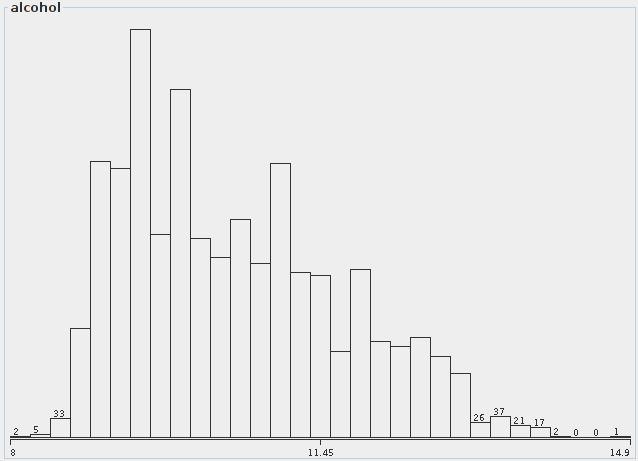
\includegraphics[width=0.6\linewidth]{img/dist-alcohol}
\caption{Data distribution of the alcohol attribute (not normalized)}
\label{fig:dist-alcohol}
\end{figure}

\begin{comment}
    \begin{figure}
    \centering
    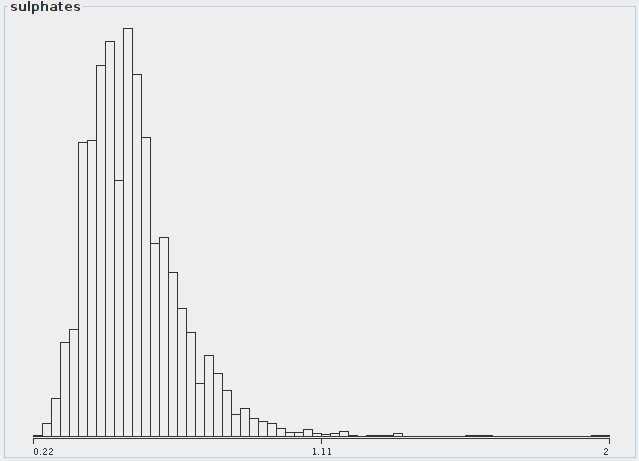
\includegraphics[width=0.6\linewidth]{img/dist-sulphates}
    \caption{Data distribution of the sulphate attribute (not normalized)}
    \label{fig:dist-sulphates}
    \end{figure}
\end{comment}


For Fixed/Volatile acidity and Total sulfur dioxide we apply Zero Mean Variance scaling. For these three we 
believe that the few outliers are features, not noise in the measurements.
For all others\footnote{Citri acid, Residual Sugar, Chlorides, Free/Total sulfur dioxide, Density, Sulphates}
we decided to exclude data samples with the outliers. The Table~\ref{tab:cutoff} shows the threshold after we drop
the data record. In Figure~\ref{fig:dist-citric-acid} a sample of the not normalized data is shown. A lot
of samples have a value to the left of the attribute range. Figure~\ref{fig:ndist-citric-acid} shows the
normalized attribute range.

\begin{figure}
\centering
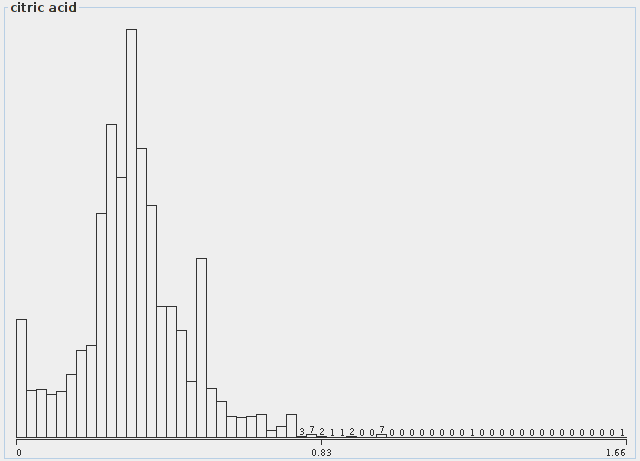
\includegraphics[width=0.6\linewidth]{img/dist-citric-acid}
\caption{Data distribution of the citric acid attribute (not normalized)}
\label{fig:dist-citric-acid}
\end{figure}

\begin{figure}
\centering
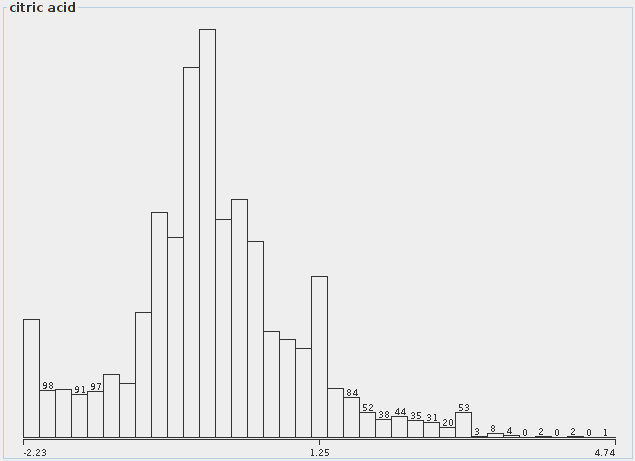
\includegraphics[width=0.6\linewidth]{img/ndist-citric-acid}
\caption{Data distribution of the citric acid attribute (normalized)}
\label{fig:ndist-citric-acid}
\end{figure}

\begin{table}
\centering
\begin{tabular}{l|c}
    Attribute & Cutoff \\
    \hline
    \hline
    Citri acid & 1.0 \\
    \hline
    Residual Sugar & 30.0 \\
    \hline
    Chlorides & 0.3 \\
    \hline
    Free sulfur dioxide & 150 \\
    \hline
    Density & 1.01 \\
    \hline
    Sulphates & 1.3 \\
\end{tabular}
\caption{Table that shows the cutoff for normalizations}
\label{tab:cutoff}
\end{table}

The total amount of rows that are filtered are 44 rows. This decreases the data set from 6497 instances to 6453.
We provide the original data samples in a file called ``wq.csv'', the samples that do not include quality and wine type
in ``wq-n-o.csv'' and the normalized data in ``wq-n.csv''.

\begin{comment}
In our automated script we used Python 2.7. To repeat the experiment we set the random seed to 0.
It cannot occur that one data sample of the original samples is included twice in the subsampled dataset.
\end{comment}
We also include the Python script called ``wine.py'' that can be invoked\footnote{Example: python wine.py < wq.csv} on the original dataset ``wq.csv'' to generate all files needed by the SOMToolbox.

\subsection{Classification}

In the original data set the attribute quality were used for classification. As we merged the white and red wine,
we additionally binned the quality into 3 bins: Poor-, Average- and High- quality. We did this, to reduce the possible
amount of clusters (6 instead of approx. 14).
The data samples included in WQ covered a range from 3 to 9. Table~\ref{tab:quality-binning} shows the binning settings.
The bins are not equally distributed along the range, but we selected them by seeing the distribution in WEKA. Nearly
all bins should have an equal amount of samples accociated to them.

\begin{table}
\centering
\begin{tabular}{l|c|c}
    Class & Quality Range & Class ID (red/white)\\
    \hline
    \hline
    Poorquality & $[0,5]$ & (0,1) \\
    \hline
    Averagequality & $[6,6]$ & (2,3) \\
    \hline
    Highquality & $[7,10]$ & (4,5) \\
    \hline
\end{tabular}
\caption{Shows the binning range for white and red wine}
\label{tab:quality-binning}
\end{table}

\section{Training the first SOM}

After we have familiarized ourselfs with the SOMToolbox we will start to train a rather small
map. We use the settings for the ``Small Map'' shown in Table~\ref{tab:settings}. If not further
noted in the description we use the standard settings.

The following list explains the settings in more detail that are shown in Table~\ref{tab:settings}.

\begin{itemize}
    \item $\alpha$ ... the learning rate
    \item $\sigma$ ... the neighbourhood radius
    \item $s_x$ ... size of the SOM grid on the x-axis
    \item $s_y$ ... size of the SOM grid on the y-axis
    \item $i$ ... the amount of iterations
\end{itemize}

For all of our experiments we prohibit the SOM Toolbox to normalize the data because we have
already done it previously.

\begin{table*}
\centering
\begin{tabular}{|l|c|c|c|c|c|c|}
    \hline
    Small Map & $\alpha = 0.7$ & $\sigma = 7$ & $s_x=5$ & $s_y=5$ & $i=1.500$ \\
    \hline
    Big Map & $\alpha = 0.7$ & $\sigma = 7$ & $s_x=50$ & $s_y=50$ & $i=1.500$ \\
    \hline
    Middle sized Map & $\alpha = 0.7$ & $\sigma = 7$ & $s_x=18$ & $s_y=18$ & $i=1.500$ \\
    \hline
    Errornous normalized Map & $\alpha = 0.7$ & $\sigma = 7$ & $s_x=20$ & $s_y=14$ & $i=1.500$ \\
    \hline
    Neighbourhood Small & $\alpha = 0.7$ & $\sigma = 1$ & $s_x=20$ & $s_y=16$ & $i=5.000$ \\
    \hline
    Neighbourhood Mid & $\alpha = 0.7$ & $\sigma = 5$ & $s_x=20$ & $s_y=16$ & $i=5.000$ \\
    \hline
    Neighbourhood Normal & $\alpha = 0.7$ & $\sigma = 10$ & $s_x=20$ & $s_y=16$ & $i=5.000$ \\
    \hline
    Neighbourhood Big & $\alpha = 0.7$ & $\sigma = 15$ & $s_x=20$ & $s_y=14$ & $i=5.000$ \\
    \hline
\end{tabular}
\caption{Settings for all of our experiments}
\label{tab:settings}
\end{table*}

\subsection{Small SOM}

We consider a $5\times5$ grid for our first experiment very small. WQ has more than 6000 entries.
This will result in many input samples grouped together to very few nodes. Our first trained
SOM is shown in Figure~\ref{fig:wine-small-hit-histogram} using the hit histogram visualization.
It can reveal dense areas on the map and in our opinion shows that the map size is too small.
We only have few units that are not fully colored in red. This is kind of a vertical line separating
the first 4 vertical units on the top left from the rest of the map. We conclude that there are
too many input samples are mapped to every unit int the SOM.

\begin{figure}
\centering
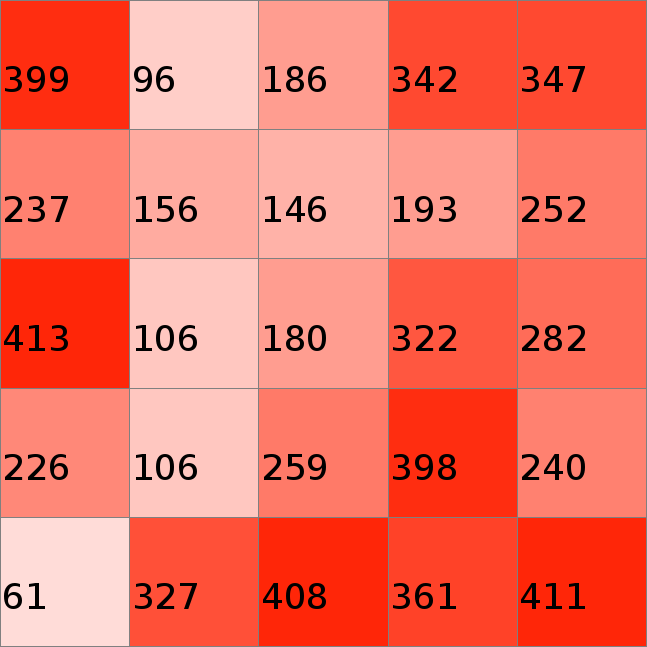
\includegraphics[width=0.5\linewidth]{img/wine-small-hit-histogram}
\caption{Hit histogram of a $5\times5$ SOM Map}
\label{fig:wine-small-hit-histogram}
\end{figure}

Another visualization hint for dense areas is the P-Matrix. It is shown in Figure~\ref{fig:wine-small-p-matrix} using
the default settings. We see that there are dense areas to the bottom right of the map and there are lesser
dense areas to the top right of the map.
By increasing the P-radius from 3 to 5 the map nearly turns into one big red pixel.
Comparing it to Figure~\ref{fig:wine-small-hit-histogram} it shows that there are many input samples densly packed
onto the lower right grid of the map. When we later increase the SOM size, this data might spread out. We
will also evaluate later to make the map rectangular because the units seem to spread into on direction.

\begin{figure}
\centering
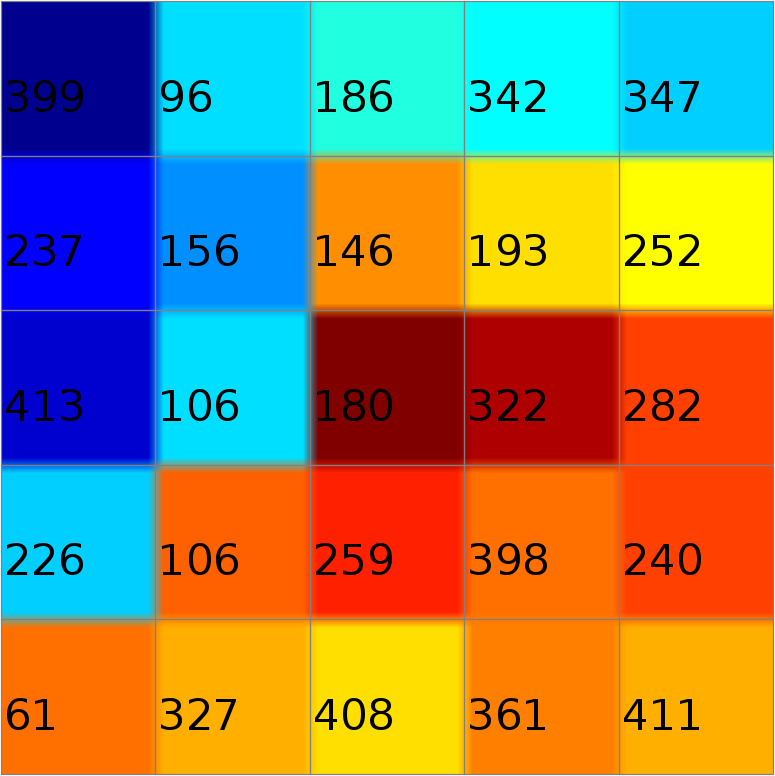
\includegraphics[width=0.5\linewidth]{img/wine-small-p-matrix}
\caption{P-Matrix Visualization of a $5\times5$ SOM Map}
\label{fig:wine-small-p-matrix}
\end{figure}

We also present the Activity Histogram of our small SOM in Figure~\ref{fig:wine-small-activity-histogram}.
Interesting is the blue part on the mid left that is separated by a slight green/yellow.
On the bottom right we again find a very dense area because of the grayish/yellow color. This this matches
well with the P-Matrix visualization. Judging from the Activity Histogram there are 2 very distinct clusters
and maybe one cluster that is very intermixed (green/yellow). This could either be that the
red and white wine are very distinct or two subranges of the quality are dominated by ranges of the input.

\begin{figure}
\centering
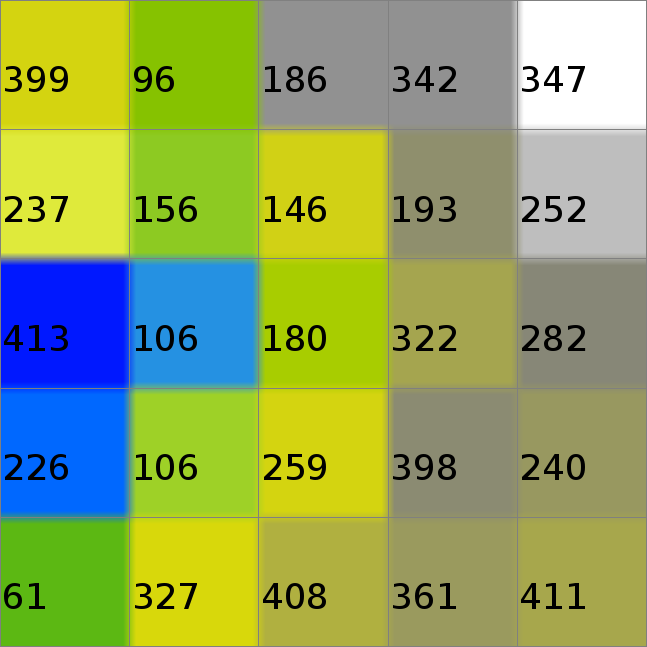
\includegraphics[width=0.5\linewidth]{img/wine-small-activity-histogram}
\caption{Activity histogram of a $5\times5$ SOM Map}
\label{fig:wine-small-activity-histogram}
\end{figure}

\subsection{Quality measurements}

In the following we take a look at some quality measures available in SOMToolbox.
If not noted otherwise the default parameter values are used for all quality measures.
First we compare the Quantization Error (QE) and the Mean Quantization Error (MQE) shown in
Figure~\ref{fig:wine-small-quant-error} and~\ref{fig:wine-small-mean-quant-error} respectivley.
We already noted that the lower right is a very dense area. In the MQE these units have a very low
MQE rate thus they are colored blue. In the QE Figure the values are much more scattered. In
the top left it has a very high value thus it seems that there is an area that is not that dense
and has many items with a long distance. This we also can confirm using the MQE, because the division
by the nodes does not set a low value the value in MQE. It also reveals that there is potentially even a more sparse
region as the node at position $1\times1$ in MQE shows.

\begin{figure}
\centering
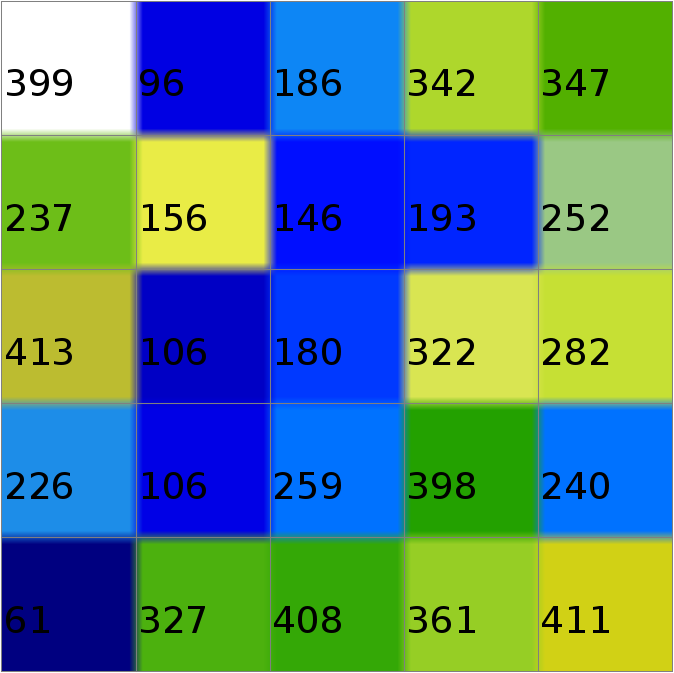
\includegraphics[width=0.5\linewidth]{img/wine-small-quant-error}
\caption{Quantization error of a $5\times5$ SOM Map}
\label{fig:wine-small-quant-error}
\end{figure}

\begin{figure}
\centering
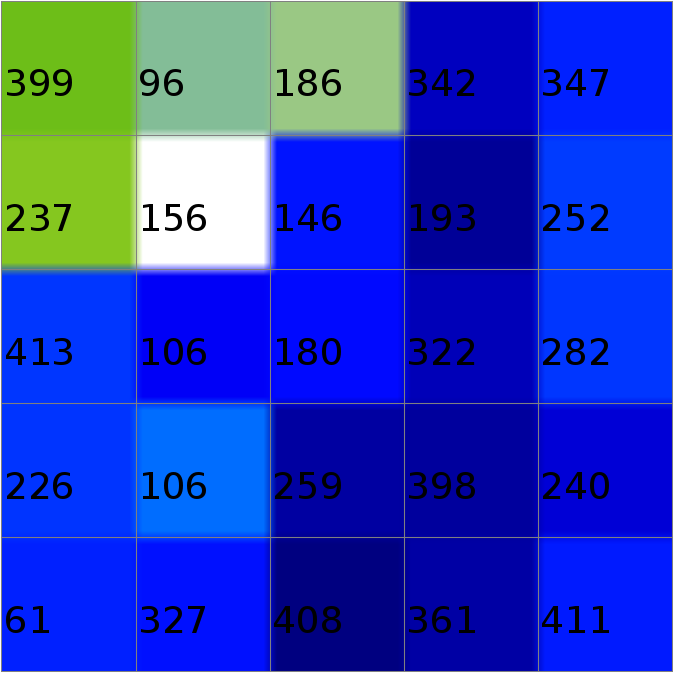
\includegraphics[width=0.5\linewidth]{img/wine-small-mean-quant-error}
\caption{Mean quantization error of a $5\times5$ SOM Map}
\label{fig:wine-small-mean-quant-error}
\end{figure}

The map is also very distorted which is shown in Figure~\ref{fig:wine-small-dist-sqrt-2}.
When comparing this to a better train map (such as the sample of Iris dataset), it is
really distorted. Given the number of values mapped to the nodes, the distortion and
high QE we conclude current SOM size is to small.

\begin{figure}
\centering
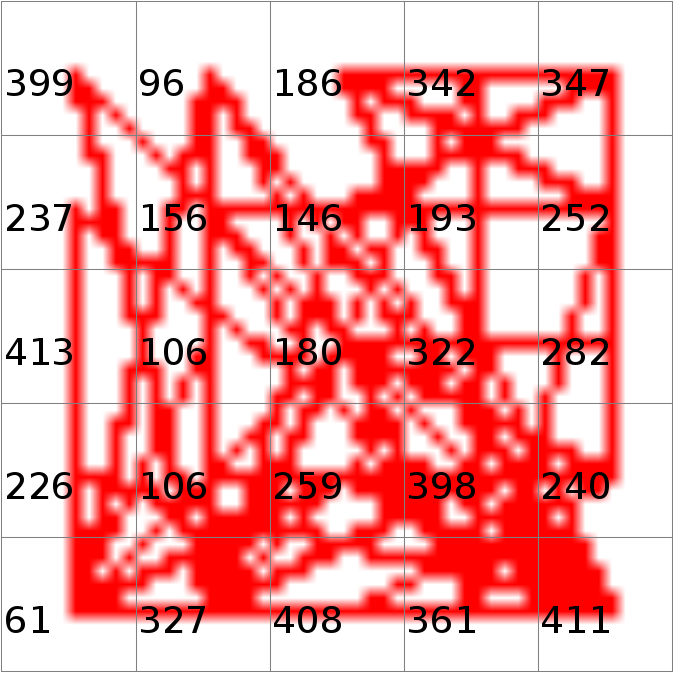
\includegraphics[width=0.5\linewidth]{img/wine-small-dist-sqrt-2}
\caption{Distoration of the map ($\sqrt{2}$) of a $5\times5$ SOM Map}
\label{fig:wine-small-dist-sqrt-2}
\end{figure}

To finish the examination of this far to small map we show the class distribution amongst the map.
At first it surprised us that the splitting is done quite evenly between red and
white wine. Giving this a second thought it is clear that they must be more easily separatable.
White and red wine have very different characteristics in sugar, acid, etc. 
White wine is colored green (light green is poor quality, green is average quality and dark green is high quality) and
red wine is colored red(light for poor quality, orange for average quality and dark for high quality).

What we also have seen in the class distribution is that white wine has far more data samples
than the red wine. Thus we apply subsampling of white wine input samples. We reduce the dataset to around 1500 red and 1500 white wine samples.
We use a random seed of 0 in our export script to repeat this experiment.

\begin{figure}
\centering
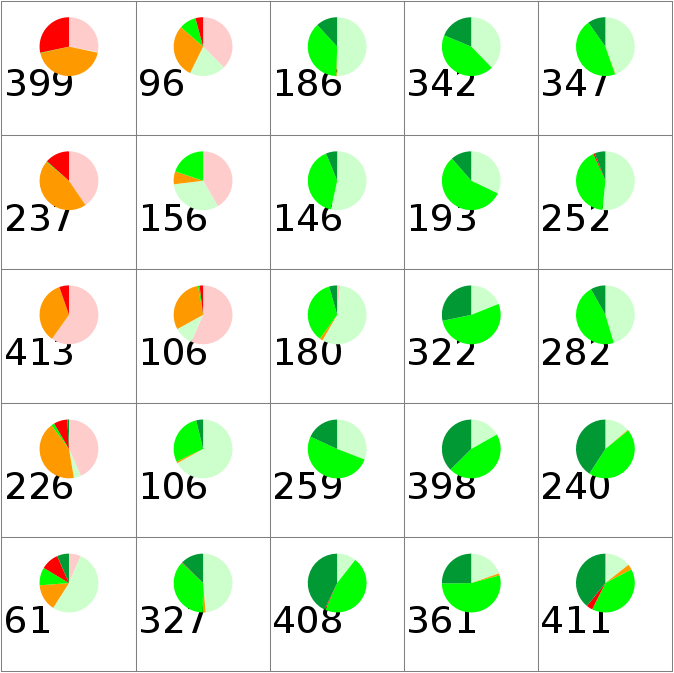
\includegraphics[width=0.5\linewidth]{img/wine-small-pie-cls}
\caption{Piechart that shows the class distribution of a $5\times5$ SOM Map}
\label{fig:wine-small-pie-cls}
\end{figure}

\section{A very big SOM}

Now we would like to examine the data in a very big SOM. The settings are displayed
in~\ref{tab:settings}. Our assumption is that it is too big if we have less than 3
samples per SOM unit.

To find out if the SOM is too big we take a look at the QE (Figure ~\ref{fig:wine-big-quant-error}) and MQE (Figure~\ref{fig:wine-big-mean-quant-error}) quality measurements.
The first thing we noticed is the huge number of interpolating/empty units on the map. By comparing QE and MQE we noticed that there is not
a significant differance in the color coding. This is caused by fact that map is too big and only a small number of samples
are mapped to the units.
At this point we immediatly stopped to evaluate this huge SOM and decreased the size to $30\times30$. The main reason was that we had problems
with the SOM Toolbox to display various visualizations. Even the $30\times30$ SOM confirms our assumption that big sized SOMs have
many interpolating units. The picture of the QE and MQE are quite the same but only with fewer nodes.


\begin{figure}
\centering
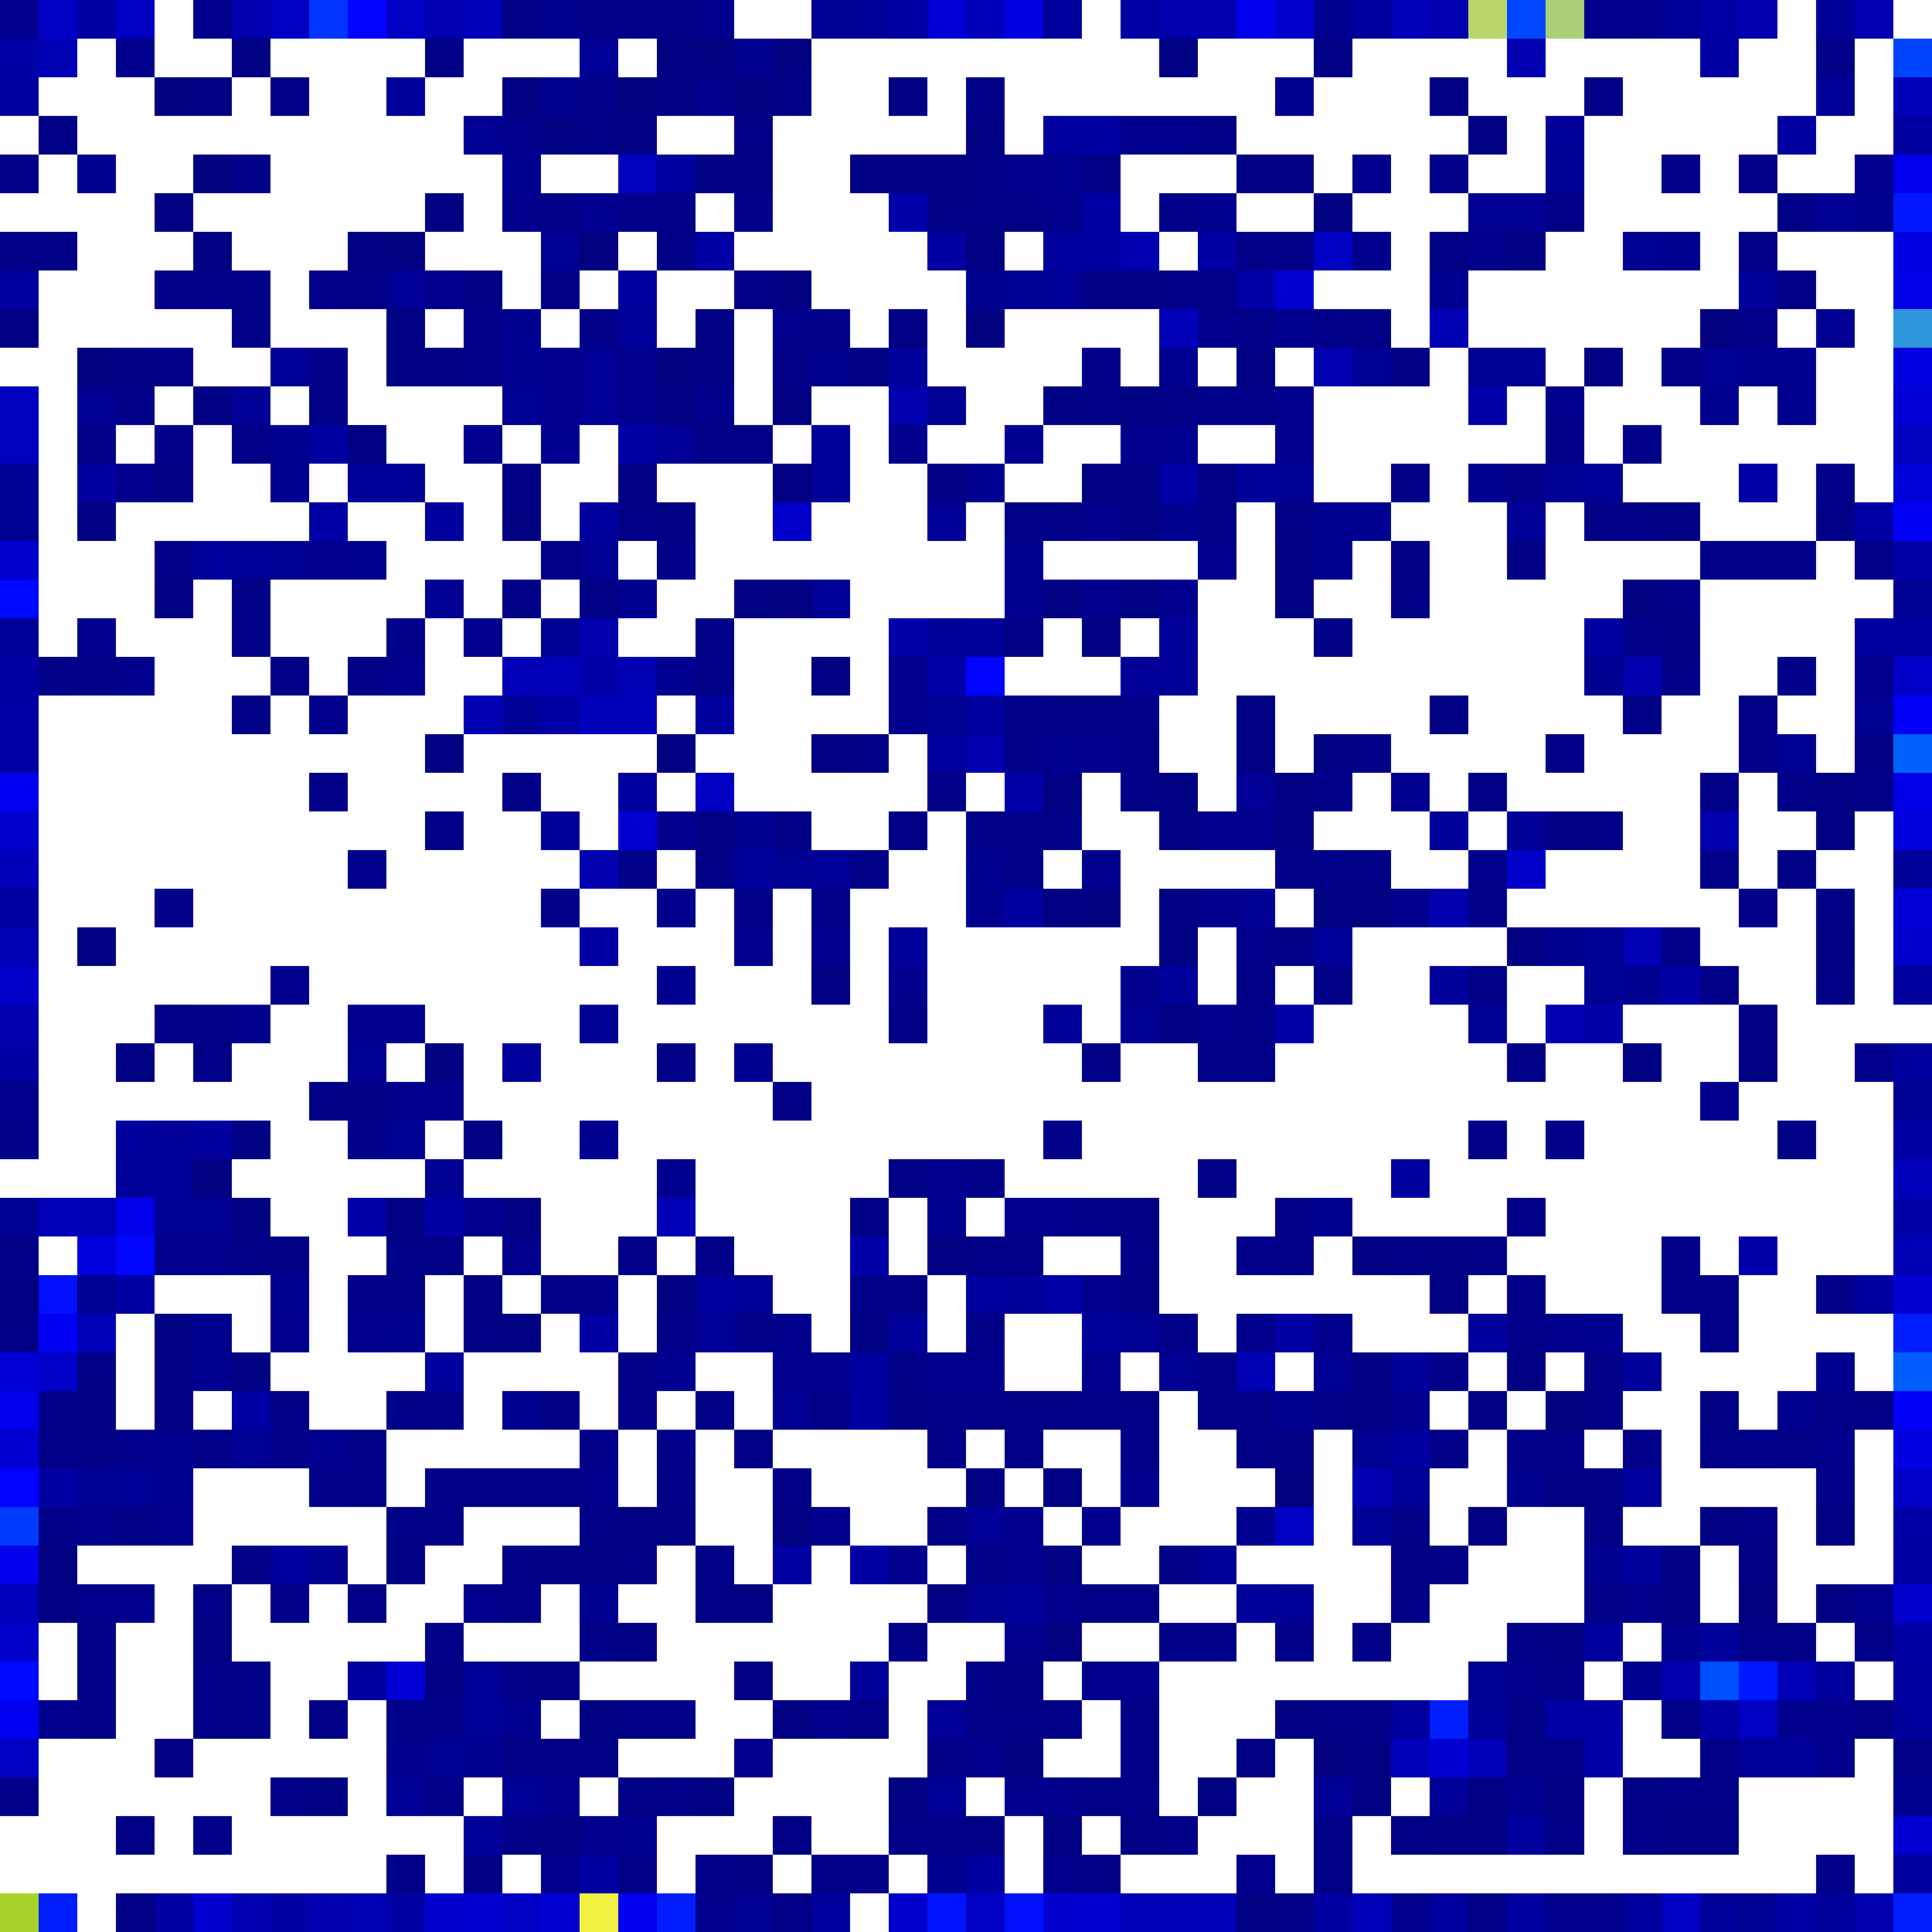
\includegraphics[width=\linewidth]{img/wine-big-quant-error}
\caption{Quantisation error of a $50\times50$ SOM Map}
\label{fig:wine-big-quant-error}
\end{figure}

\begin{figure}
\centering
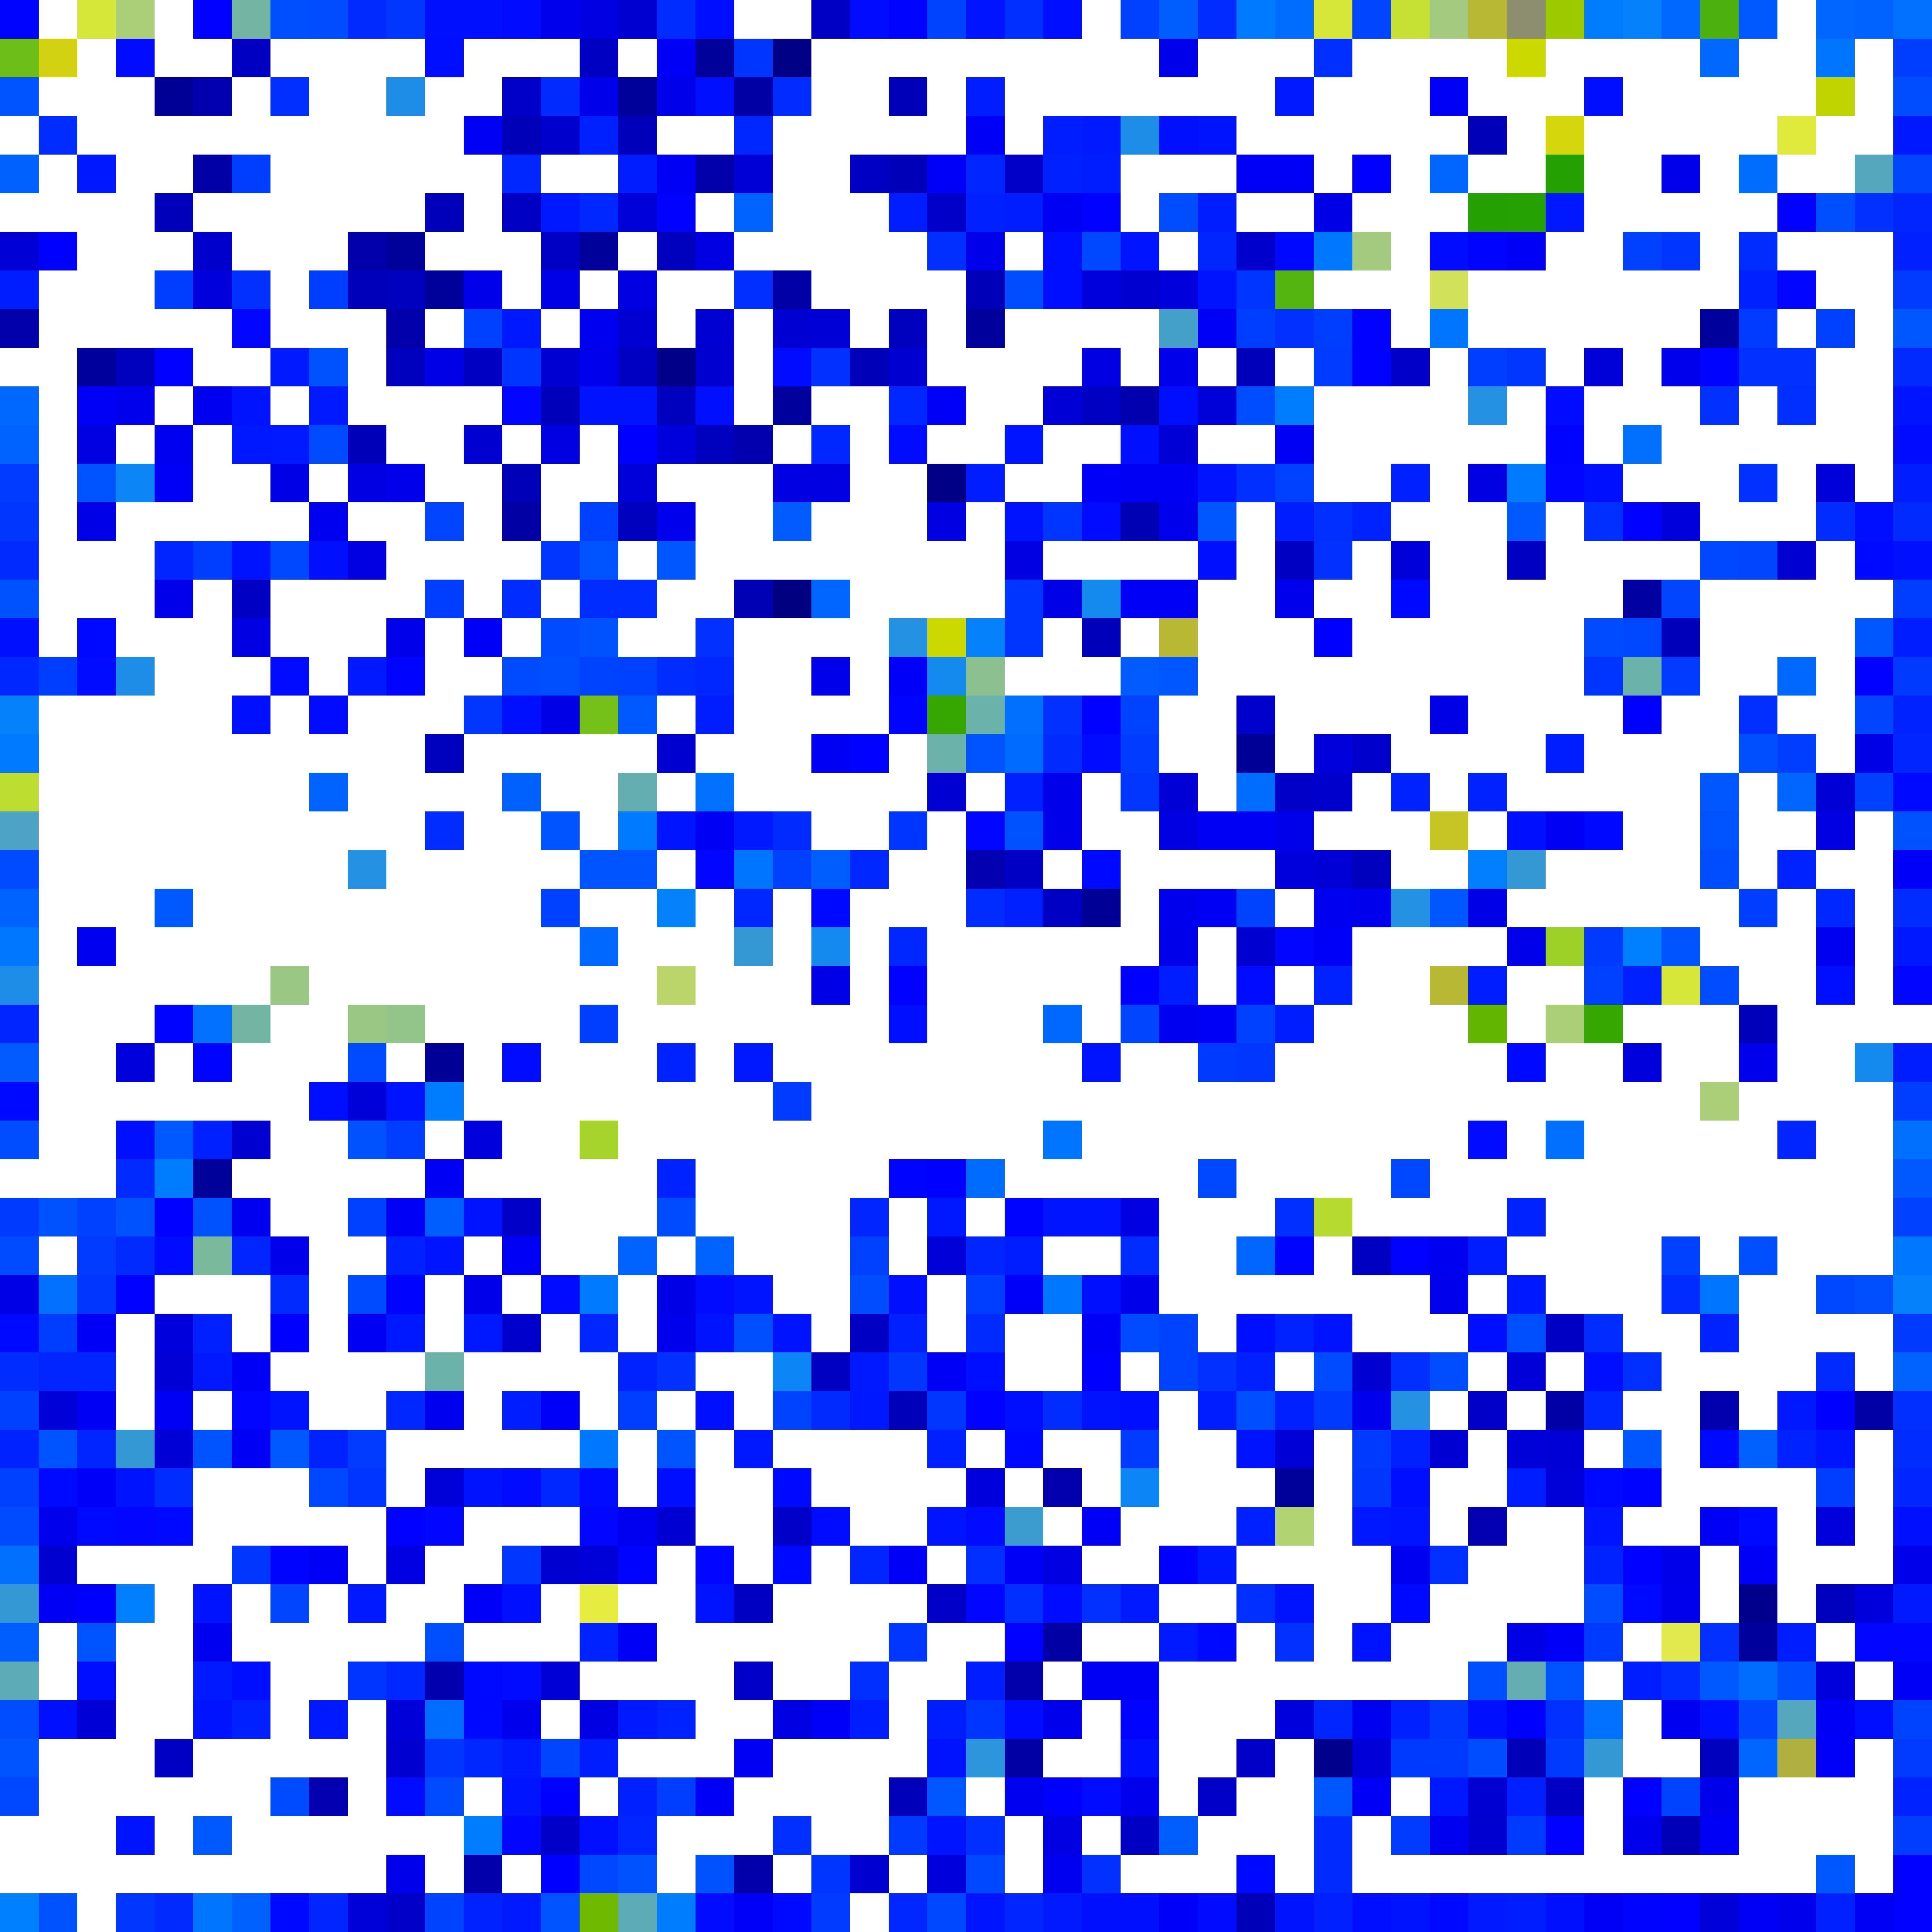
\includegraphics[width=\linewidth]{img/wine-big-mean-quant-error}
\caption{Quantisation error of a $50\times50$ SOM Map}
\label{fig:wine-big-mean-quant-error}
\end{figure}

We assume that the hit histogram of the $50\times50$ SOM should not have alot of red spots.
Using the hit histogram of the smaller big SOM ($30\times30$) shown in Figure~\ref{fig:wine-big-hit-histogram} we notice that very light
colors which indicates that few or none input samples are mapped to the SOM nodes.

\begin{figure}
\centering
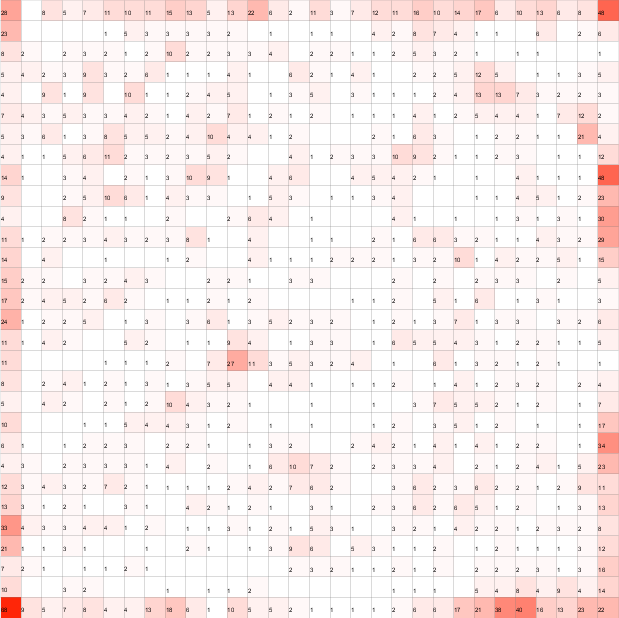
\includegraphics[width=\linewidth]{img/wine-big-hit-histogram}
\caption{Hit histogram of a $30\times30$ SOM Map}
\label{fig:wine-big-hit-histogram}
\end{figure}

In Figure~\ref{wine-big-p-matrix} we se a huge red spot in the center of the map. This indicates that
the data is very dense at this area. Comparing it to the small SOM P-Matrix there is this dense area
in the center. The difference is that the dense area is to the center right not to the bottom right as assumed with
the small one.

\begin{figure}
\centering
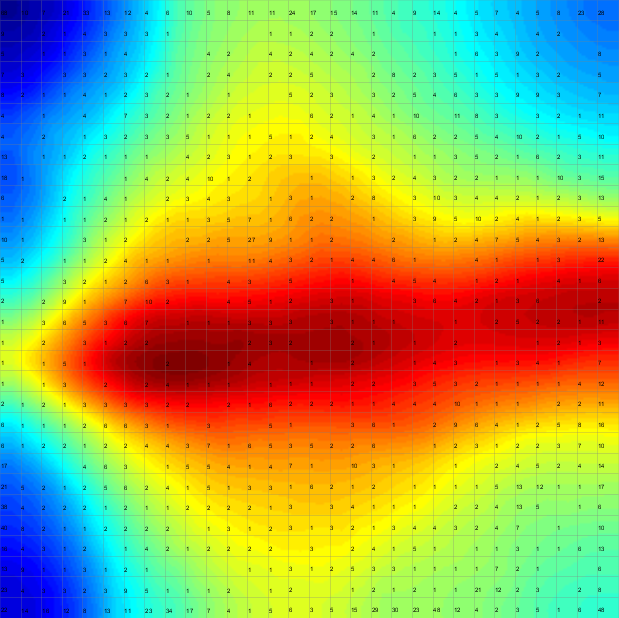
\includegraphics[width=\linewidth]{img/wine-big-p-matrix}
\caption{P matrix visualization of a $30\times30$ SOM Map}
\label{fig:wine-big-p-matrix}
\end{figure}

The last quality measure we apply for this map is the topographic product.
We used a setting of $k=1$. The visualisation reveals a distortion in the
SOM borders and a horizontal line of distortion in the center of the map.
When increasing the number of neighbours ($k$) we still see the distortion
we mentioned earlier.

\begin{figure}
\centering
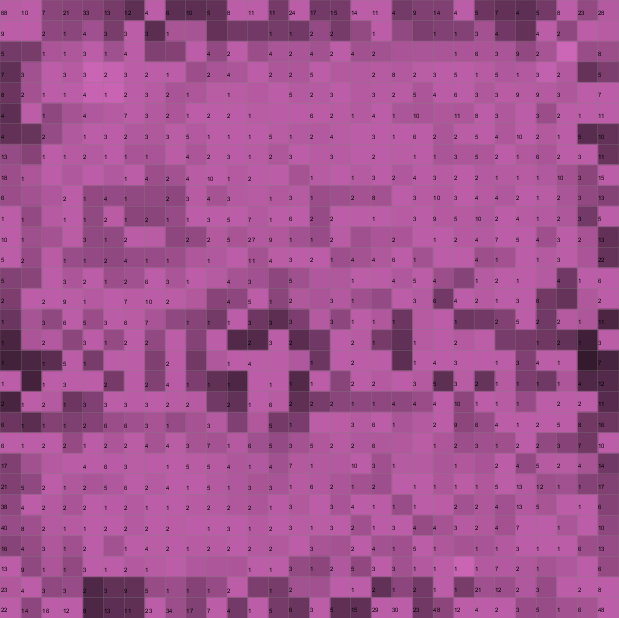
\includegraphics[width=\linewidth]{img/wine-big-topo-product}
\caption{Topographic product of the $30\times30$ SOM Map}
\label{fig:wine-big-topo-product}
\end{figure}

In the Figure~\ref{fig:wine-big-u-matrix} we show the U-Matrix visualization.
It reveals the possible cluster bounderies. We have many coherent regions/valleys located in
the upper and lower parts of the map. They are separated by a horizontal mountain regions
or high values in the center which depict the possible cluster boundaries.

\begin{figure}
\centering
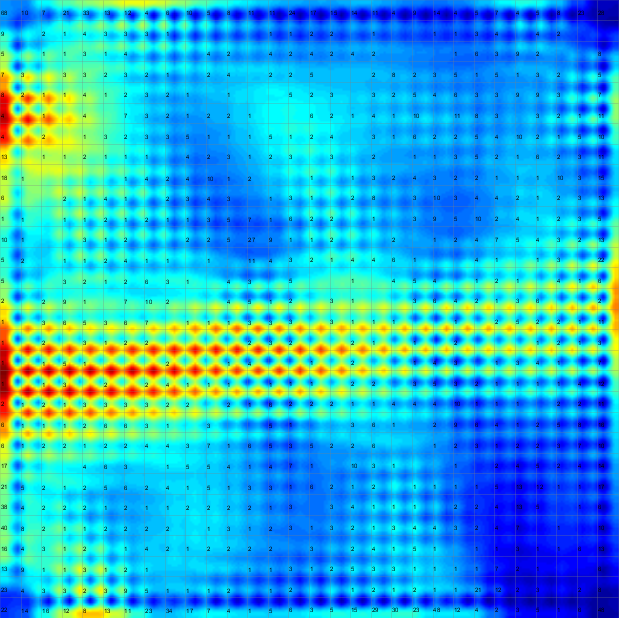
\includegraphics[width=\linewidth]{img/wine-big-u-matrix}
\caption{U Matrix of the $30\times30$ SOM Map}
\label{fig:wine-big-u-matrix}
\end{figure}

The potential cluster boundaries displayed in the SDH visualization in Figure~\ref{fig:wine-big-smoothed-data-histogram}.

\begin{figure}
\centering
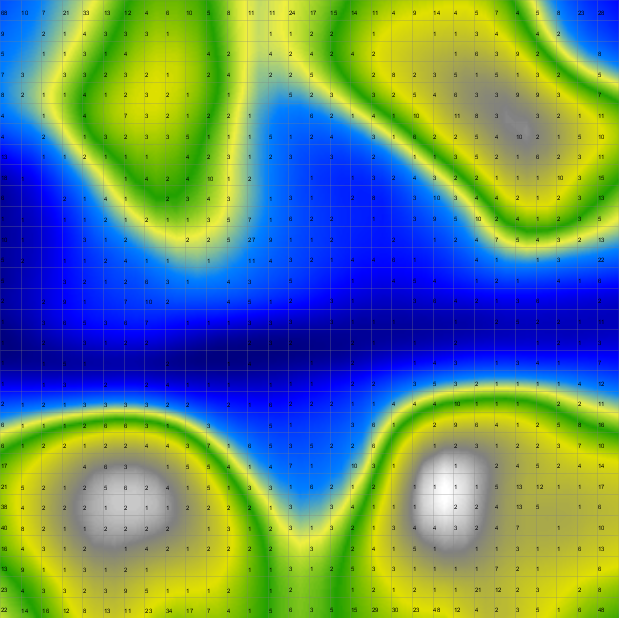
\includegraphics[width=\linewidth]{img/wine-big-smoothed-data-histogram}
\caption{Smoothed data histograms of the $30\times30$ SOM Map}
\label{fig:wine-big-smoothed-data-histogram}
\end{figure}

In addition the activity historygram in Figure~\ref{fig:wine-big-activity-histogram} shows possible
topology violations. There is not a gradient of the weight vectors measured in distance. In can
be seen in the upper cluster where blue area is separated by green.

\begin{figure}
\centering
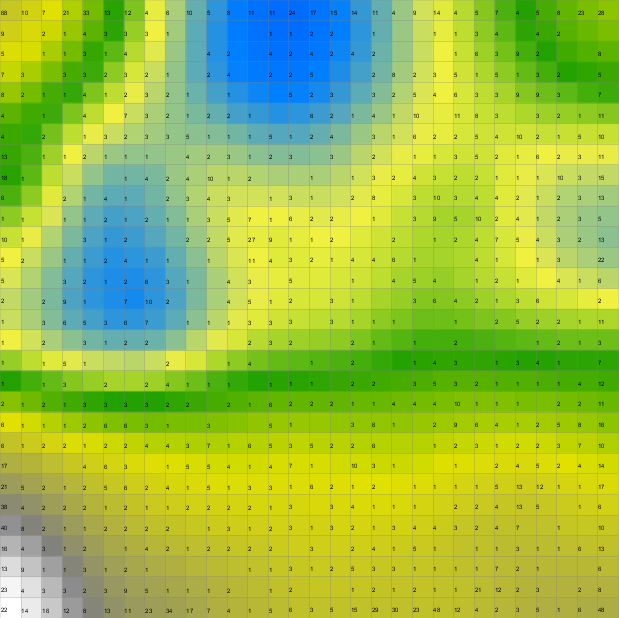
\includegraphics[width=\linewidth]{img/wine-big-activity-histogram}
\caption{Activity histogram of the $30\times30$ SOM Map}
\label{fig:wine-big-activity-histogram}
\end{figure}

The analysed visulations/quality measures depict that we SOM is oversized.
In the following we will try to approximate a better size.

\section{Normal SOM}

In the following we show a middle sized map. Parameters are included in the Table~\ref{tab:settings}.
On the first view of QE in Figure~\ref{fig:wine-mid-quant-error} and MQE~\ref{fig:wine-mid-quant-error} we see
that there are three interpolating units. Comparing the two we notice that the distant data samples are
mapped to the units located along the a horzontal line in the center or the potential cluster boundaries.
The U-Matrix in Figure~\ref{fig:wine-mid-u-matrix} reveals the cluster bounderies shown with high mountain values
along the line mentioned earlier.

Again we used the SDH visualization. In the earlier settings we used a smoothing factor of 149. We decreased it to
115 and managed to separate the two main clusters shown in Figure~\ref{fig:wine-mid-soothed-data-histogram}.

There are potential topology violations located in the upper cluster. We see this in Figure~\ref{fig:wine-mid-activity-histogram}.
Like in the big SOM there are three blue areas separated by green an yellow. By observing the neighbourhood graph
shown in Figure~\ref{fig:wine-mid-radius-neighbourhood-grah}. For the radius was set to 0.4. We notice three red lines connecting the blue areas.


\begin{figure}
\centering
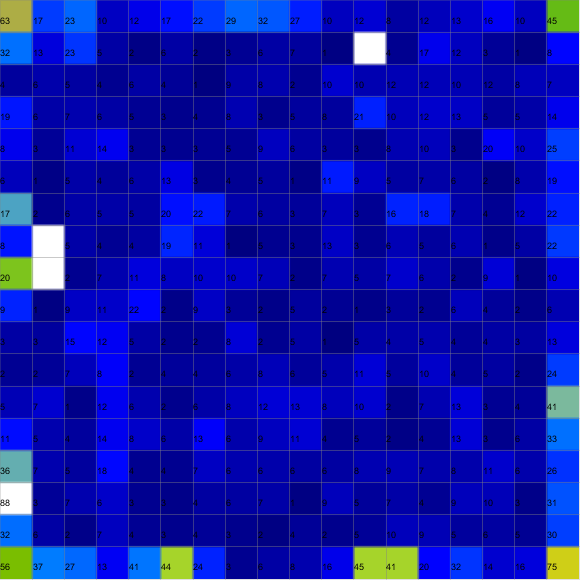
\includegraphics[width=\linewidth]{img/wine-mid-quant-error}
\caption{Quantisation error of a $18\times18$ SOM Map}
\label{fig:wine-mid-quant-error}
\end{figure}

\begin{figure}
\centering
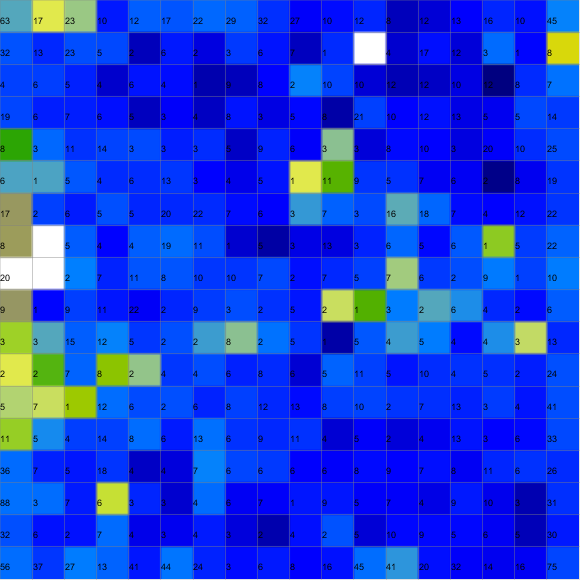
\includegraphics[width=\linewidth]{img/wine-mid-mean-quant-error}
\caption{Quantisation error of a $18\times18$ SOM Map}
\label{fig:wine-mid-mean-quant-error}
\end{figure}

\begin{figure}
\centering
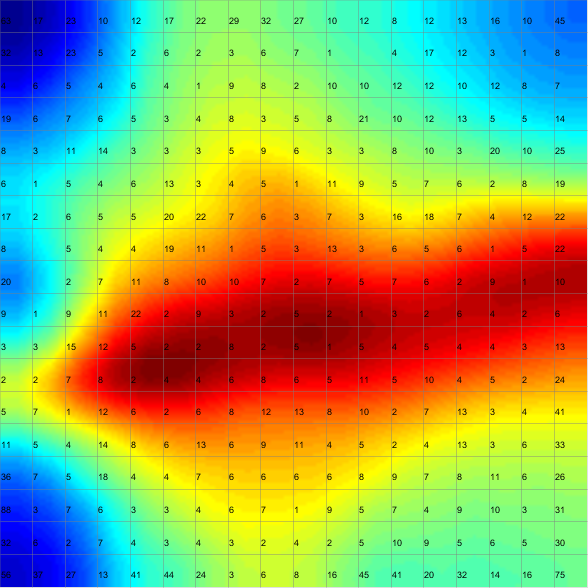
\includegraphics[width=\linewidth]{img/wine-mid-p-matrix}
\caption{P matrix visualization of a $18\times18$ SOM Map}
\label{fig:wine-mid-p-matrix}
\end{figure}

\begin{figure}
\centering
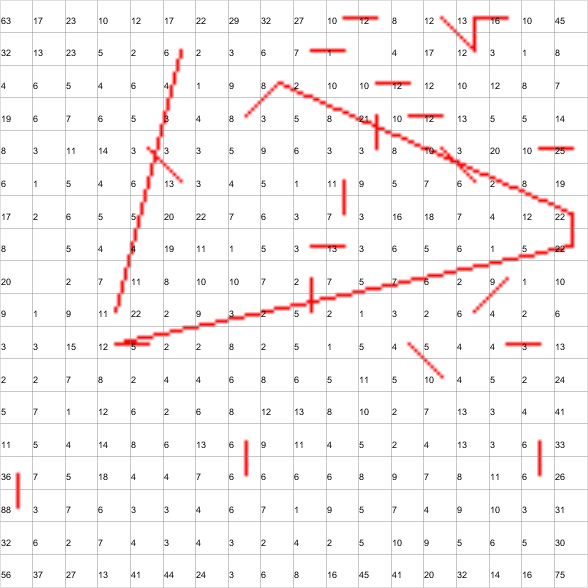
\includegraphics[width=\linewidth]{img/wine-mid-radius-neighbourhood-graph}
\caption{Topographic product of the $18\times18$ SOM Map}
\label{fig:wine-mid-radius-neighbourhood-graph}
\end{figure}

\begin{figure}
\centering
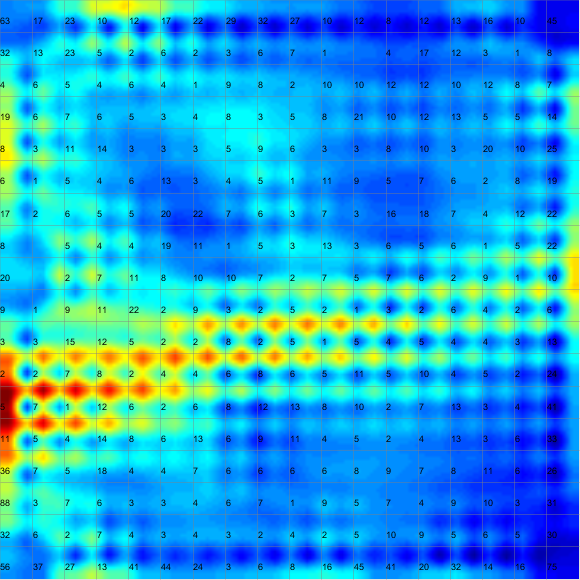
\includegraphics[width=\linewidth]{img/wine-mid-u-matrix}
\caption{U Matrix of the $18\times18$ SOM Map}
\label{fig:wine-mid-u-matrix}
\end{figure}

\begin{figure}
\centering
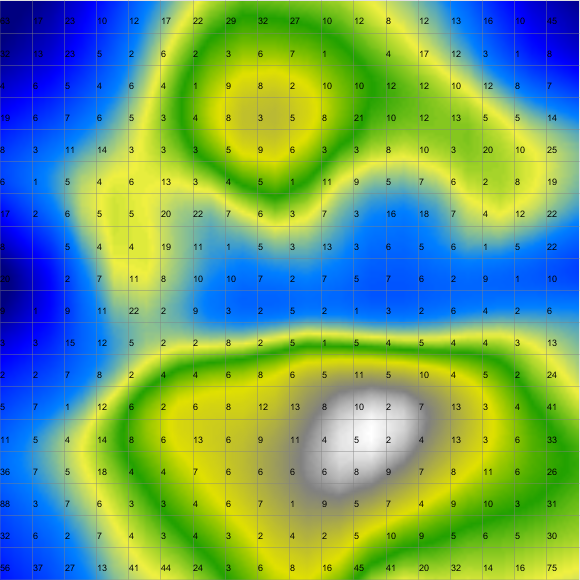
\includegraphics[width=\linewidth]{img/wine-mid-smoothed-data-histogram}
\caption{Smoothed data histograms of the $18\times18$ SOM Map}
\label{fig:wine-mid-smoothed-data-histogram}
\end{figure}

\begin{figure}
\centering
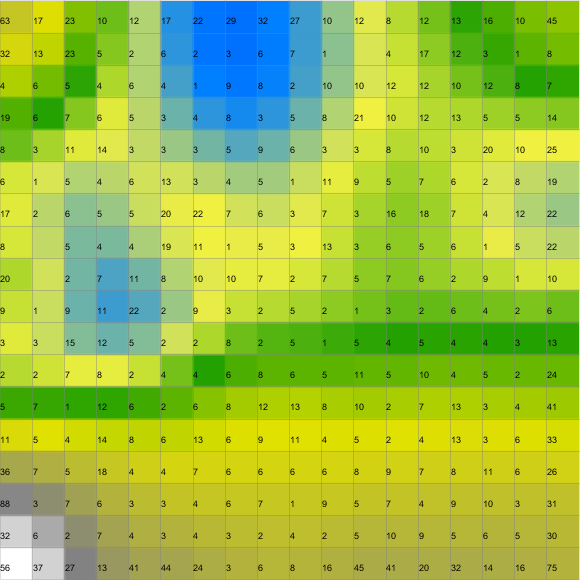
\includegraphics[width=\linewidth]{img/wine-mid-activity-histogram}
\caption{Activity histogram of the $18\times18$ SOM Map}
\label{fig:wine-mid-activity-histogram}
\end{figure}

\section{SOM random Initialization. Different Seed values}
As discovered in the previous analysis, the rectangular SOM clearly contains critical Topology 
violations in the right area. We tried to improve the mapping quality by training a SOM 
with hexagonal structure and as shown on Activity histogram of the hexagonal SOM in FIGURE 
we managed to merge the a group of similar weight vectors colored with blue in one area 
instead of being separated as by green weight vectors as shown in FIGURE of the rectangular SOM.
The hexagonal SOM was trained with the default initial parameters as shown in TABLE. Further
to our analysis, we trained two additional SOM with identical initial parameters but with 
different random initializations by specific different seed values. As noted before, we discovered
two main clusters and by observing the Activity Histogram we can notice the movement of the clusters.
For Seed=1 the right cluster is weak but as we change increase the seed values to Seed =7 we notice
clearer definition of the blue area and then for seed=55 we observe complete cluster shift.
The U-Matrix shows that for Seed=1 the cluster boundaries are vertical but not clearly defined,
for Seed=7 they are adjusted and clear whereas for Seed=55 we observe a complete cluster boundaries
shift into a horizontal position. New discoveries of the clusters shift are revealed by the
Radius based Neighbourhood graphs by observing graphs with different radiuses r=0,5;0,8 and 1. 
For Seed 55 the rotation of the cluster boundaries is confirmed. For values we notice 
one more smaller inner cluster shift for r=0,8 on FIGURE and FIGURE. The dense area of the Right 
cluster is moved to the lower right area of the SOM. Additional finding is that for Seed=1 and
r=0.5 as shown in FIGURE we observe parable lines which are indicators of Topology Violations.


\section{SOM Normalization. Training not normalized data}

To highlight the difference between a SOM that is trained with erroneous normalized data
we use the settings provided in the Table~\ref{tab:settings}. We found out earlier that a rectangular
SOM is more useful for our data distribution. Thus we now take a look at a $20\times14$ SOM.

As we have discussed earlier, there are attributes that contain outliers.
For those\footnote{Residual Sugar, Chlorides, Free sulfur dioxide, Total sulfur dioxide, Sulphates} we apply min/max scaling. We assume that by using this scaling technique we distort these attributes, which leads to a blur of the two clusters.
For all others we use unit length scaling. As we heard in the lecture this scaling technique
divides by the vector length, thus it makes the attribute vector unit length. This is
not desirable, because we do not want our measurements to look the same. It would
make sense for an attribute like document size, because it is mostly not the document
size that defines the type of content. This is not the case for measurements.

In the following we present the Activity Histogram in Figure~\ref{fig:wine-weird-activity-histogram},
the Smoothed Data Histogram in Figure~\ref{fig:wine-weird-smoothed-data-histogram},
the U Matrix in Figure~\ref{fig:wine-weird-u-matrix} and
the Nearest Neighbourhood visualization using a radius of 0.1 in Figure~\ref{fig:wine-weird-nearest-neighbour-radius}.

\begin{figure}
\centering
    \centering
    \begin{subfigure}[b]{0.45\linewidth}
        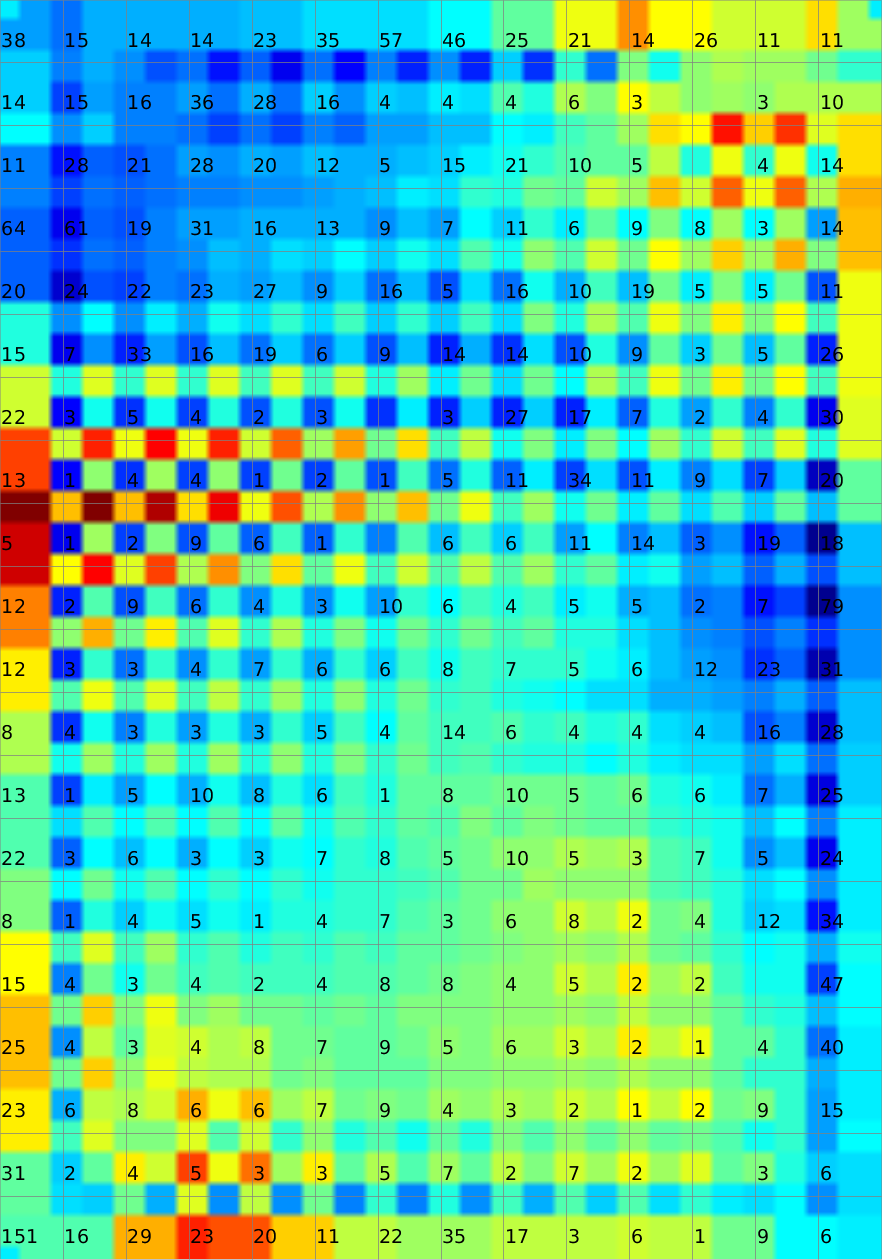
\includegraphics[width=\linewidth]{img/wine-weird-u-matrix}
        \caption{U Matrix}
        \label{fig:wine-weird-u-matrix}
    \end{subfigure}
    \begin{subfigure}[b]{0.45\linewidth}
        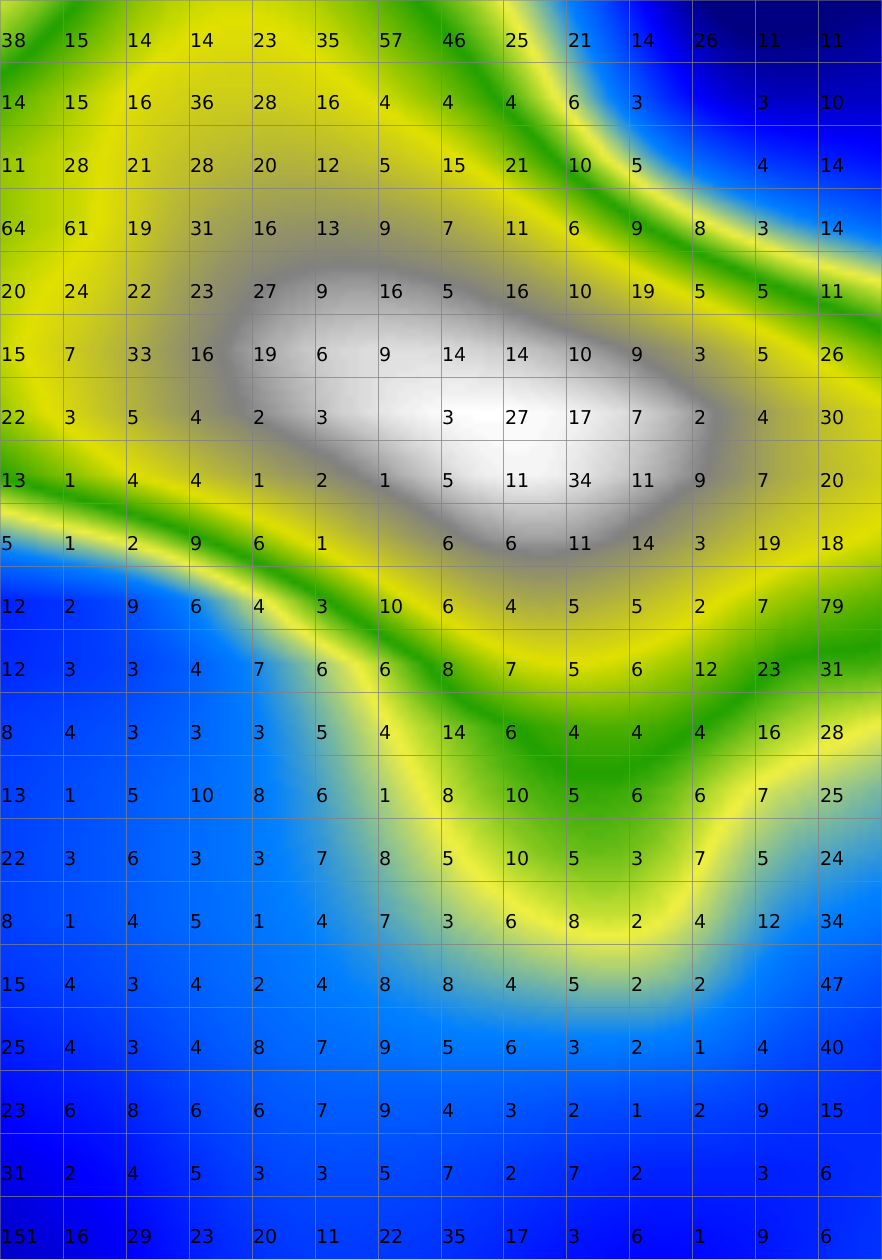
\includegraphics[width=\linewidth]{img/wine-weird-smoothed-data-histogram}
        \caption{SDH smooth factor 149}
        \label{fig:wine-weird-smoothed-data-histogram}
    \end{subfigure}
    \caption{SOM Visualisations of errornous normalized data}
\end{figure}

Comparing the U Matrix to the previous U Matrices this one has many more mountain
areas. The distinction between clusters and cluster boundaries are not visible.
In the top left there is one coherent valley that is mostly colored blue.
The rest of the map seems not to display any clusters. This is very different, because
earlier we had a clear distinction between two clusters, but here the mountains
take up to more than 80\% of the map.

The Activity Histogram now displays one gradient from the bottom left to the top right.
In the correctly normalized data we do not have such a gradient, and one part of our map
also contained topology violations.

The SDH shows very one big area located above in the center. Use a smoothing factor of 149.
When decreasing the smoothing factor the big bulb above the center is still dominant,
but moves into the top left of the map (shown in Figure~\ref{fig:wine-weird-smoothed-data-histogram-series}).
This matches very well the flat vally found in
Figure~\ref{fig:wine-weird-u-matrix}.

The nearest neighbour shows that the units of the SOM are very close to each other. The 
radius is set to 0.1. The picture shows that they are so close together, that
nearly every unit is connected to every other unit.

\begin{figure}
    \centering
    \begin{subfigure}[b]{0.45\linewidth}
        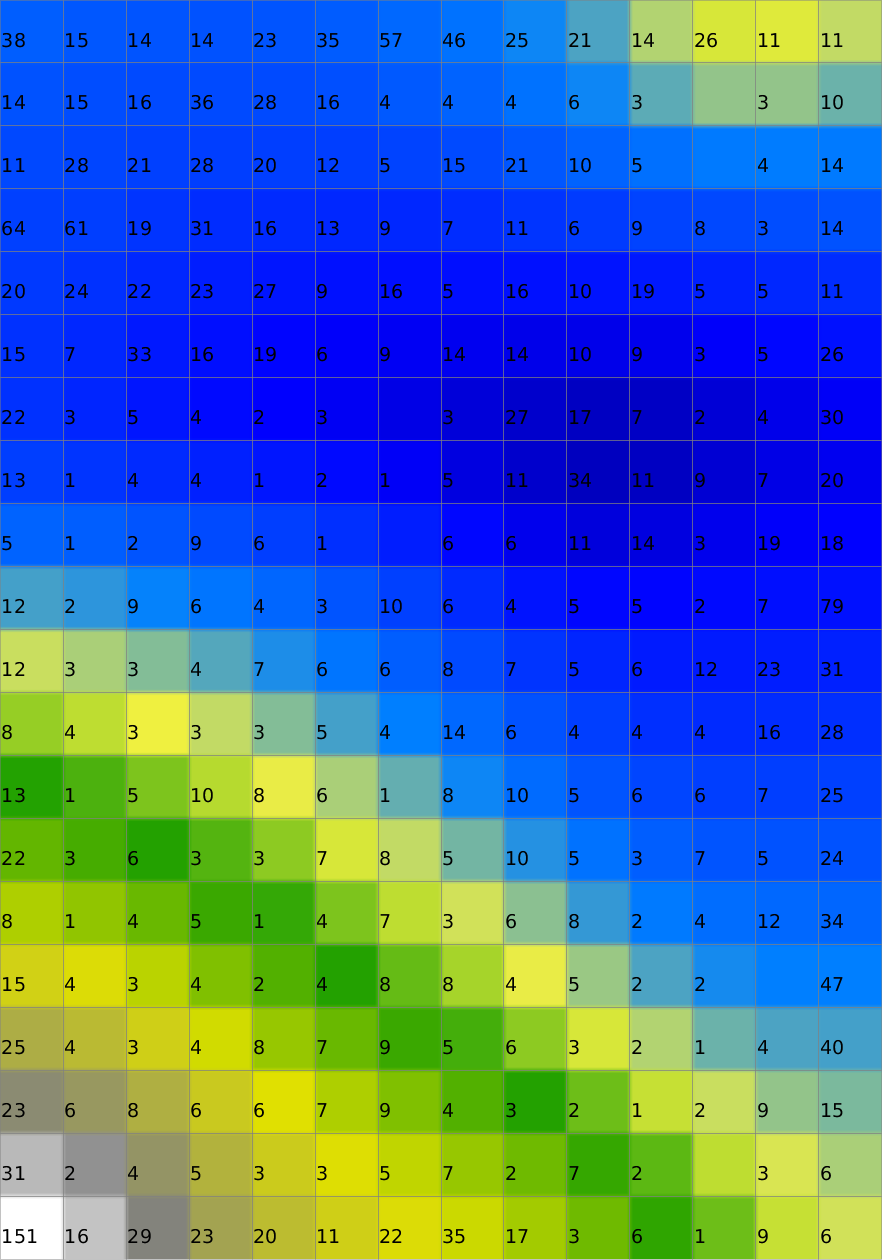
\includegraphics[width=\linewidth]{img/wine-weird-activity-histogram}
        \caption{Activity histogram}
        \label{fig:wine-weird-activity-histogram}
    \end{subfigure}
    \begin{subfigure}[b]{0.45\linewidth}
        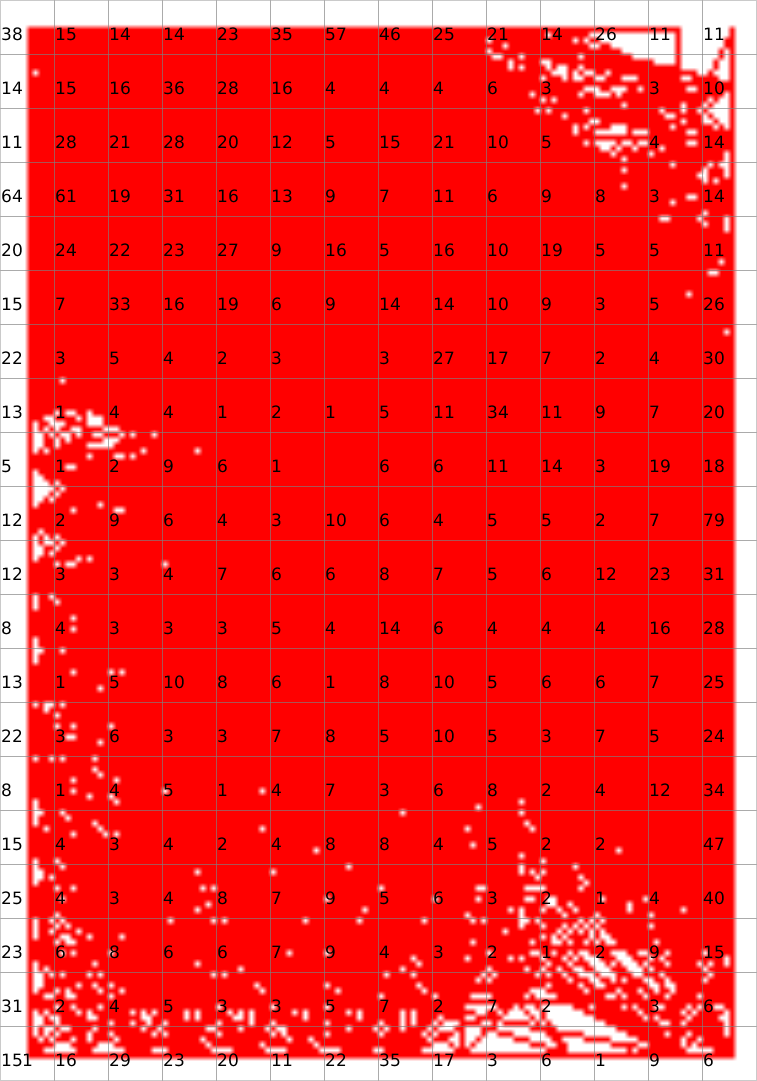
\includegraphics[width=\linewidth]{img/wine-weird-nearest-neighbour-radius}
        \caption{Nearest neighbour (radius 0.1)}
        \label{fig:wine-weird-nearest-neighbour-radius}
    \end{subfigure}
    \caption{SOM ($20\times14$) visualisations of errornous normalized data}
\end{figure}

The scaling we applied earlier was quite effective to distort the input data
and map the input data to data that looks very similar. In our opinion
many characteristics of the attributes where lost and we could verify this
in the produced SOM Visualisations.

\begin{figure}
\centering
    \centering
    \begin{subfigure}[b]{0.30\linewidth}
        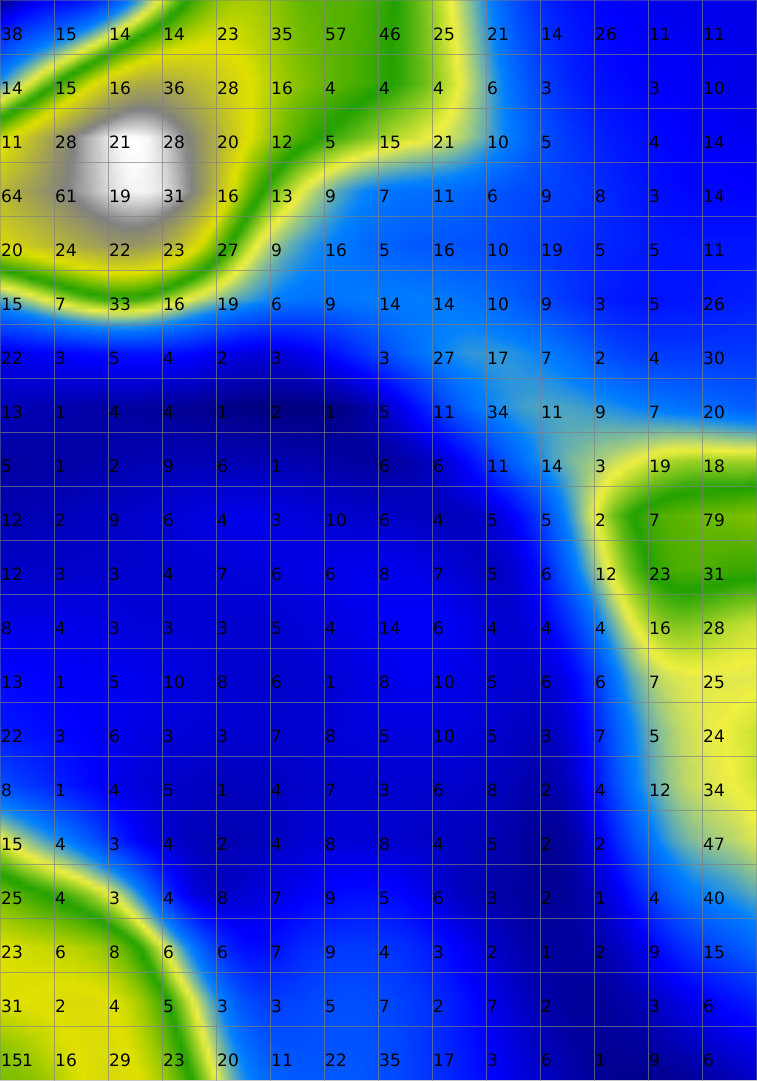
\includegraphics[width=\linewidth]{img/wine-weird-smoothed-data-histogram-20}
        \caption{$f=20$}
    \end{subfigure}
    \begin{subfigure}[b]{0.30\linewidth}
        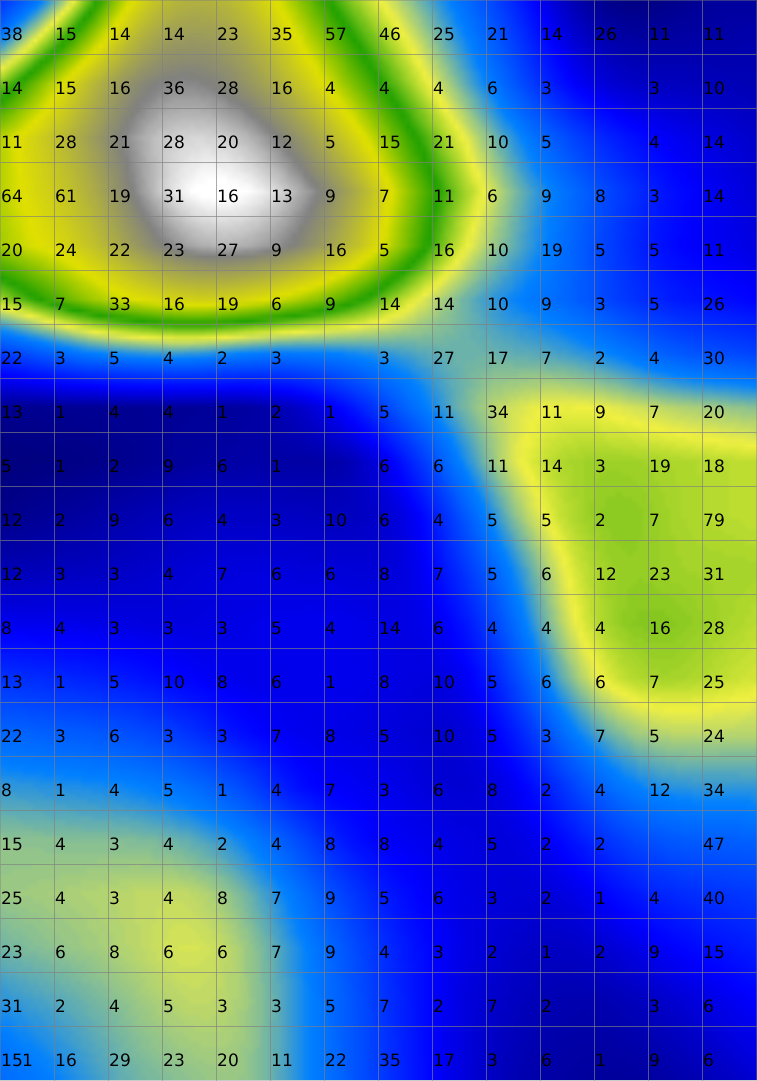
\includegraphics[width=\linewidth]{img/wine-weird-smoothed-data-histogram-50}
        \caption{$f=50$}
    \end{subfigure}
    \begin{subfigure}[b]{0.30\linewidth}
        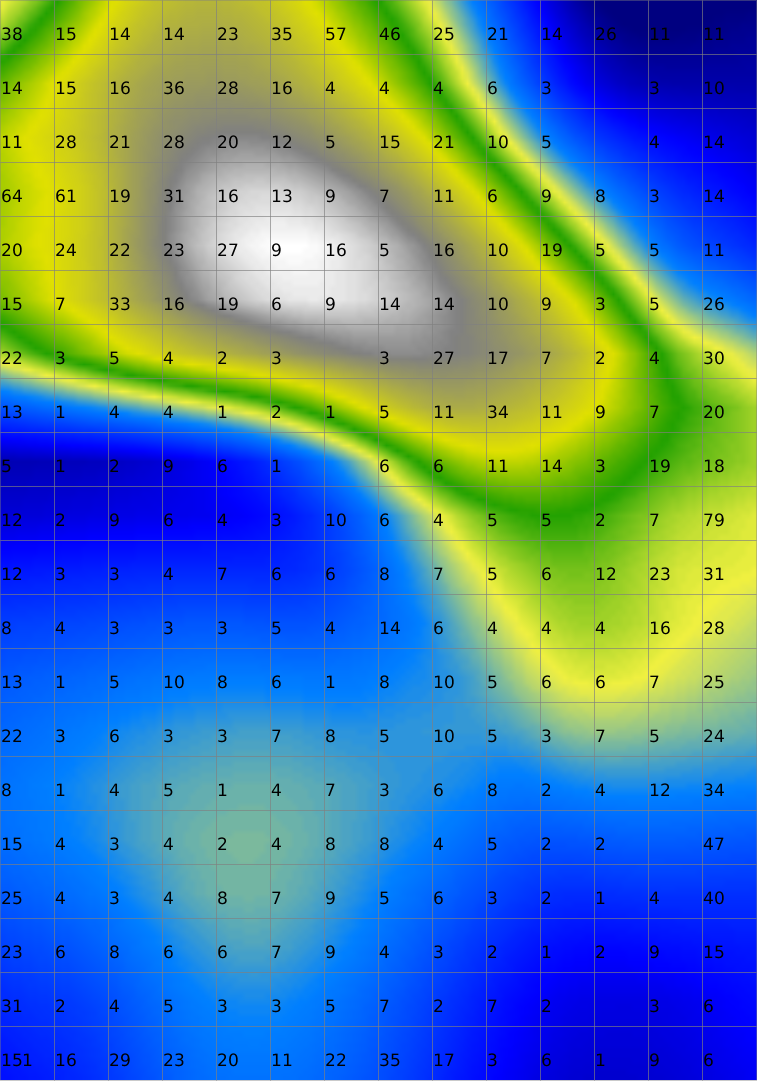
\includegraphics[width=\linewidth]{img/wine-weird-smoothed-data-histogram-100}
        \caption{$f=100$}
    \end{subfigure}
    \caption{SOM ($20\times14$) SDH with different smoothing factor $f$}
    \label{fig:wine-weird-smoothed-data-histogram-series}
\end{figure}

\section{Adjusting the neighbourhood for training}

In the following we show how the neighbourhood radius $\sigma$ affects the topology
and the structures on the map. We use the settings shown in Table~\ref{tab:settings}.
(Neighbourhood Small to Big).
For the SDH we used a smoothing factor of 100 instead of the default one.


\begin{figure}
\centering
    \centering
    \begin{subfigure}[b]{0.30\linewidth}
        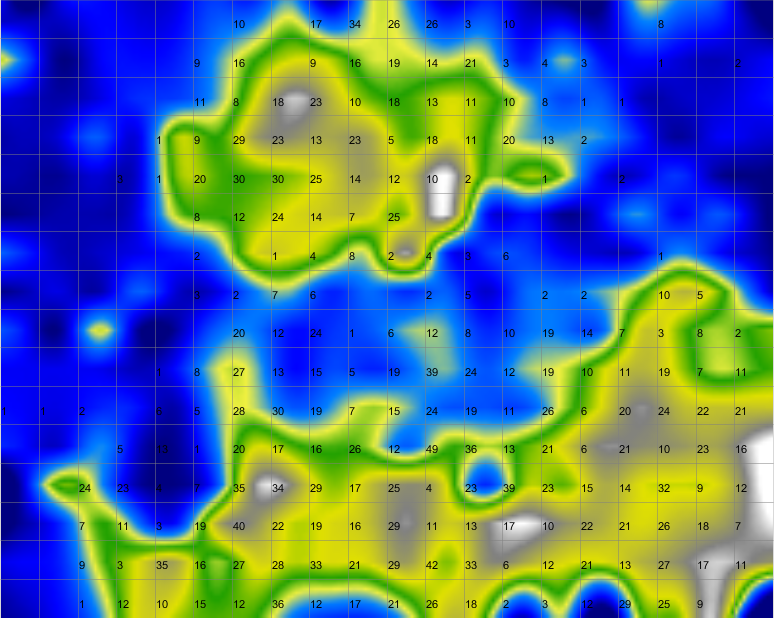
\includegraphics[width=\linewidth]{img/wine-newmid-smoothed-data-histogram-sigma-1}
        \caption{$\sigma=1$}
    \end{subfigure}
    \begin{subfigure}[b]{0.30\linewidth}
        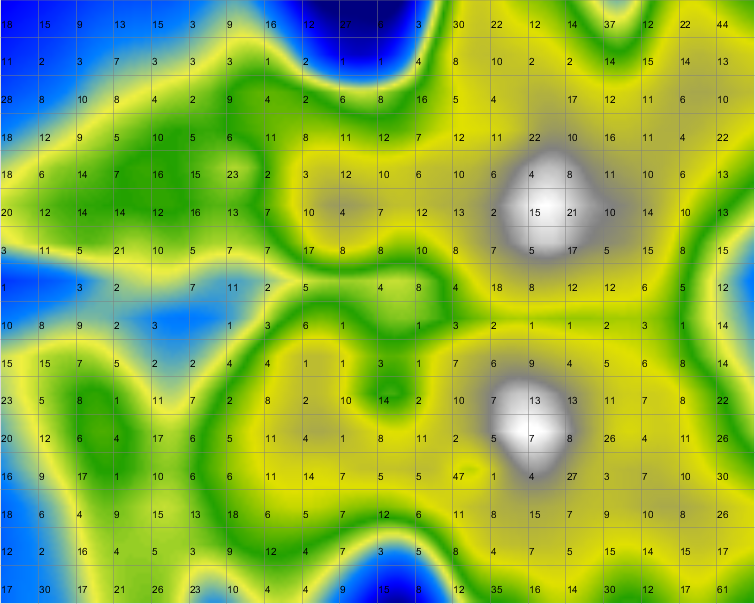
\includegraphics[width=\linewidth]{img/wine-newmid-smoothed-data-histogram-sigma-5}
        \caption{$\simga=5$}
    \end{subfigure}
    \begin{subfigure}[b]{0.30\linewidth}
        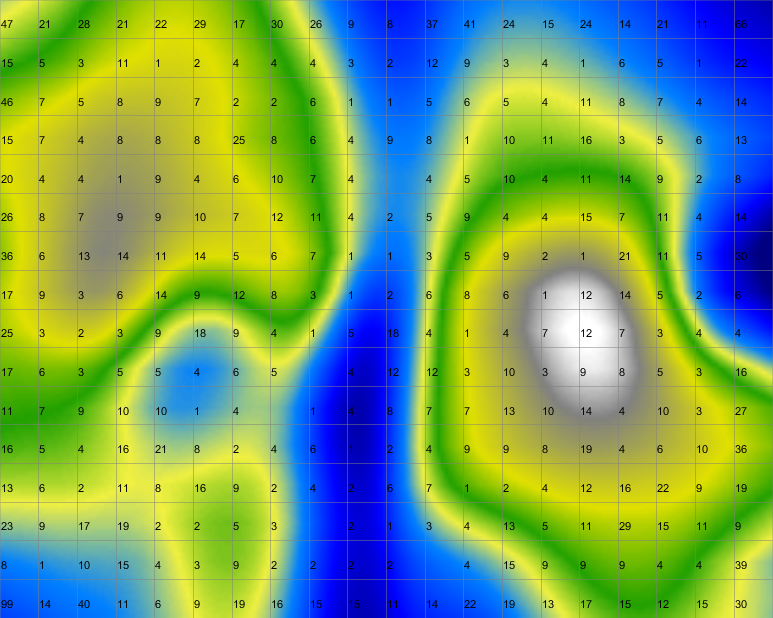
\includegraphics[width=\linewidth]{img/wine-newmid-smoothed-data-histogram-sigma-15}
        \caption{$\sigma=15$}
    \end{subfigure}
    \caption{SOM ($20\times16$) SDH with different neighbour hood radius$f$}
    \label{fig:wine-newmid-smoothed-data-histogram-sigma}
\end{figure}

\begin{figure}
\centering
    \centering
    \begin{subfigure}[b]{0.30\linewidth}
        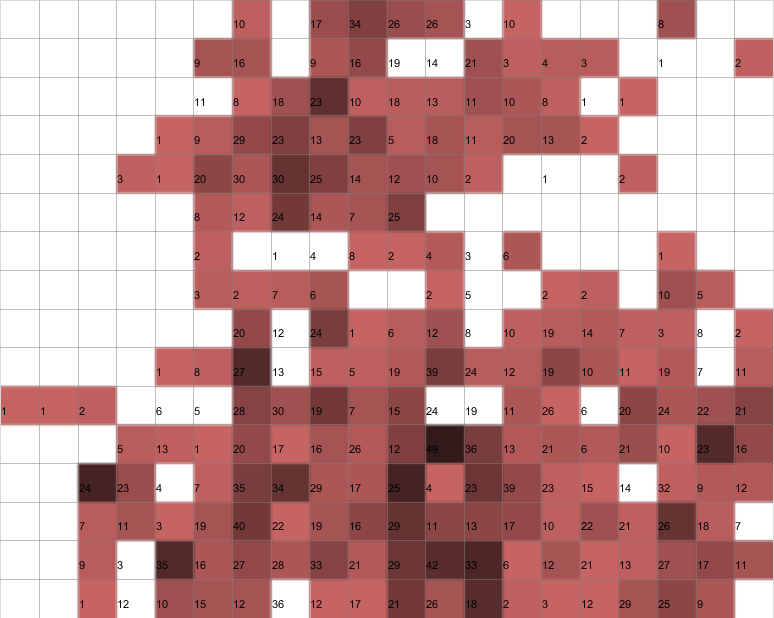
\includegraphics[width=\linewidth]{img/wine-newmid-topographic-error-sigma-1}
        \caption{$\sigma=1$}
    \end{subfigure}
    \begin{subfigure}[b]{0.30\linewidth}
        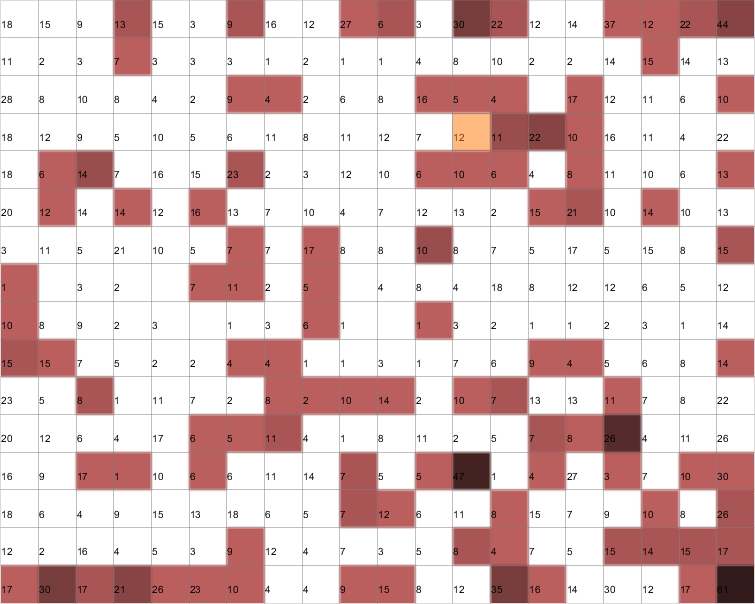
\includegraphics[width=\linewidth]{img/wine-newmid-topographic-error-sigma-5}
        \caption{$\simga=5$}
    \end{subfigure}
    \begin{subfigure}[b]{0.30\linewidth}
        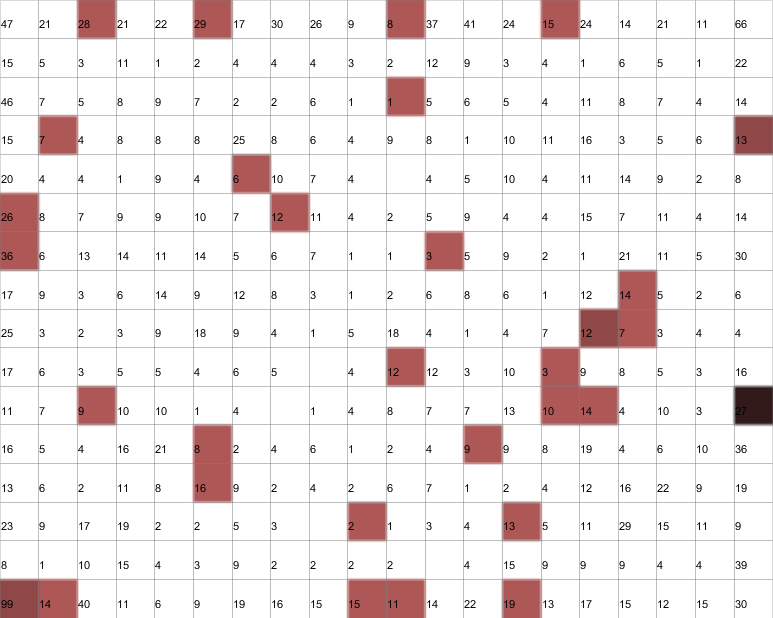
\includegraphics[width=\linewidth]{img/wine-newmid-topographic-error-sigma-15}
        \caption{$\sigma=15$}
    \end{subfigure}
    \caption{SOM ($20\times16$) Topographic error with different neighbour hood radius$f$}
    \label{fig:wine-newmid-topographic-error-sigma}
\end{figure}

\begin{figure}
\centering
    \centering
    \begin{subfigure}[b]{0.30\linewidth}
        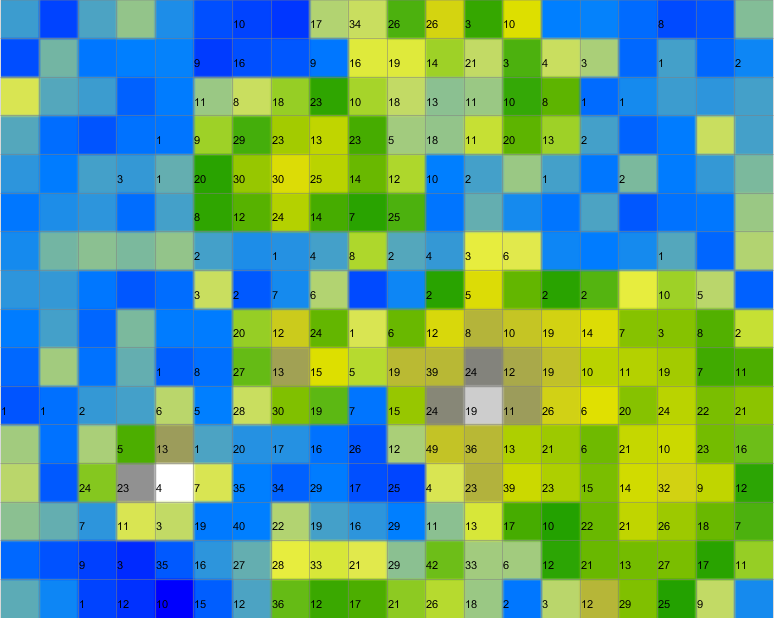
\includegraphics[width=\linewidth]{img/wine-newmid-activity-histogram-sigma-1}
        \caption{$\sigma=1$}
    \end{subfigure}
    \begin{subfigure}[b]{0.30\linewidth}
        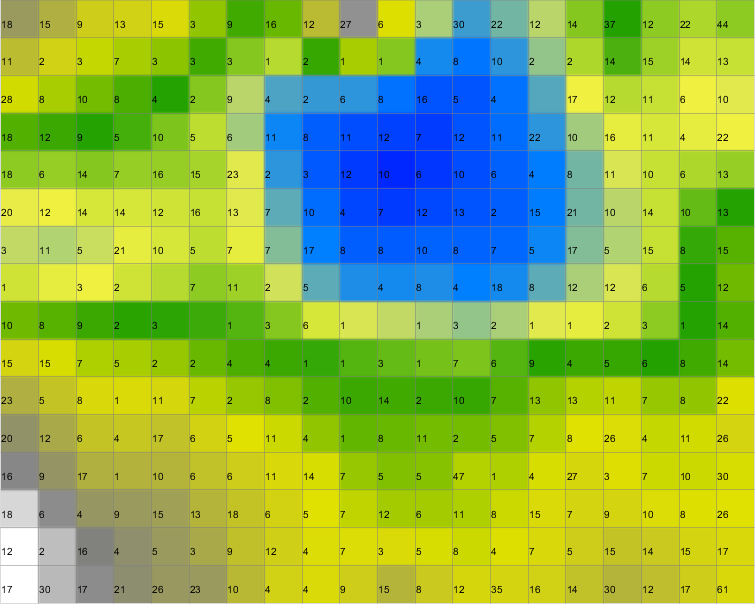
\includegraphics[width=\linewidth]{img/wine-newmid-activity-histogram-sigma-5}
        \caption{$\simga=5$}
    \end{subfigure}
    \begin{subfigure}[b]{0.30\linewidth}
        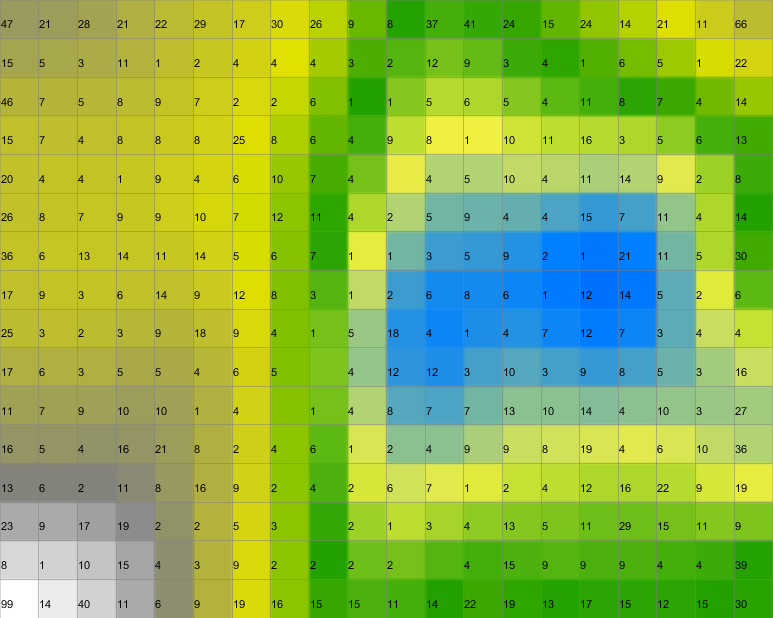
\includegraphics[width=\linewidth]{img/wine-newmid-activity-histogram-sigma-15}
        \caption{$\sigma=15$}
    \end{subfigure}
    \caption{SOM ($20\times16$) Topographic error with different neighbour hood radius$f$}
    \label{fig:wine-newmid-activity-histogram-sigma}
\end{figure}

\begin{figure}
\centering
    \centering
    \begin{subfigure}[b]{0.30\linewidth}
        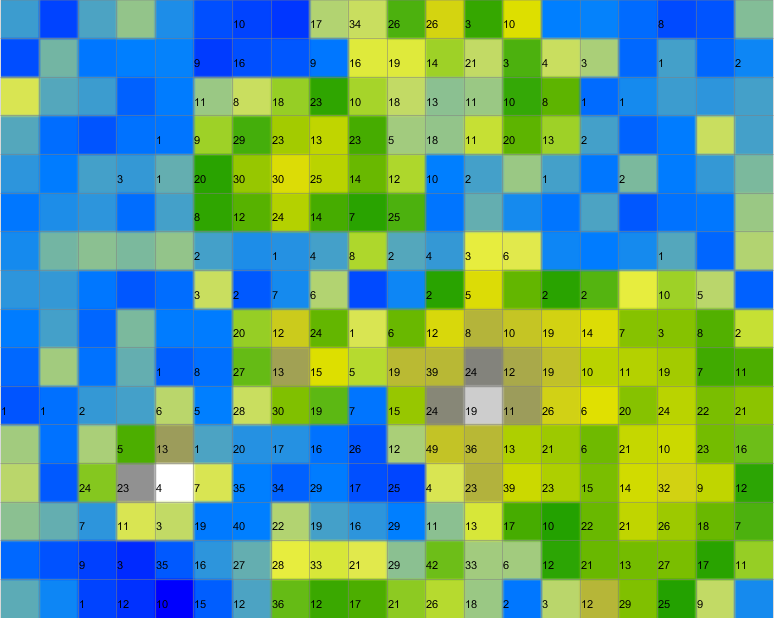
\includegraphics[width=\linewidth]{img/wine-newmid-activity-histogram-sigma-1}
        \caption{$\sigma=1$}
    \end{subfigure}
    \begin{subfigure}[b]{0.30\linewidth}
        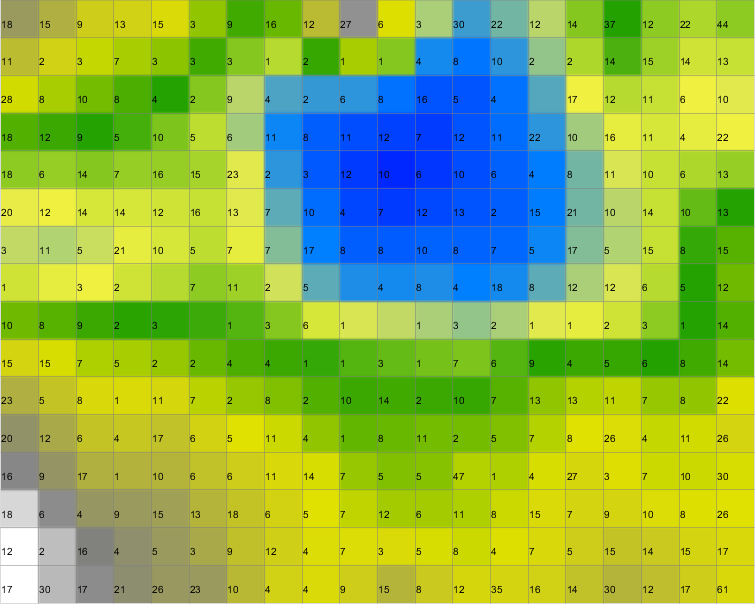
\includegraphics[width=\linewidth]{img/wine-newmid-activity-histogram-sigma-5}
        \caption{$\simga=5$}
    \end{subfigure}
    \begin{subfigure}[b]{0.30\linewidth}
        \includegraphics[width=\linewidth]{img/wine-newmid-activity-histogram-sigma-14}
        \caption{$\sigma=15$}
    \end{subfigure}
    \caption{SOM ($20\times16$) Topographic error with different neighbour hood radius$f$}
    \label{fig:wine-newmid-activity-histogram-sigma}
\end{figure}

\bibliography{ref}
\bibliographystyle{plain}



\end{document}
